\documentclass{report_template_oxford}

\title{3YP Report}
\subtitle{Multiagent Autonomous Drone System for Landmine Detection}
\author{Group B: Huirui Dai, Samuel Grace, Rory Millard, Jihwan Shin, Thomas Turner}
\date{March 2025}

\begin{document}
\maketitle

\newacronym{ATL}{ATL}{anti-tank landmine}
\newacronym{APL}{APL}{anti-personnel landmine}
\newacronym{EMI}{EMI}{Electromagnetic Induction}
\newacronym{IR}{IR}{infrared}
\newacronym{IR}{IR}{infrared}
\newacronym{USD}{USD}{United States Dollar}
\newacronym{GBP}{GBP}{Great Britain Pound}
\newacronym{LWIR}{LWIR}{long-wave infrared}
\newacronym{TNT}{TNT}{trinitrotoluene}
\newacronym{FOV}{FOV}{field of view}
\newacronym{IFOV}{IFOV}{instantaneous field of view}
\newacronym{GSD}{GSD}{ground sample distance}
\newacronym{NIR}{NIR}{near-infrared}
\newacronym{SWIR}{SWIR}{short-wave infrared}
\newacronym{MWIR}{MWIR}{mid-wave infrared}
\newacronym{FIR}{FIR}{far-infrared}
\newacronym{NETD}{NETD}{Noise Equivalent Temperature Difference}
\newacronym{SNR}{SNR}{signal-to-noise ratio}
\newacronym{COTS}{COTS}{commercial off-the-shelf}
\newacronym{EM}{EM}{electromagnetic}
\newacronym{SAR}{SAR}{Syntheic Aperture Radar}
\newacronym{ADC}{ADC}{analog-to-digital converter}
\newacronym{FMCW}{FMCW}{Frequency-Modulated Continuous Wave}
\newacronym{SFCW}{SFCW}{Stepped-Frequency Continuous Wave}
\newacronym{BP}{BP}{Back-Projection}
\newacronym{FLGPR}{FLGPR}{Forward-Looking Ground Penetrating Radar}
\newacronym{DLGPR}{DLGPR}{Down-Looking Ground Penetrating Radar}
\newacronym{SDR}{SDR}{Software Defined Radio}
\newacronym{GPR}{GPR}{Ground Penetrating Radar}

\include{Thomas/thomas_header}

% Abstract
% - Concise summary of report
% - Naming of essential outcomes
% - As short as possible while providing key points
% - Less than 1 page
\pagenumbering{roman}
\newpage
\addcontentsline{toc}{section}{Abstract}
\fancyhead[C]{Rory Millard}
\section*{Abstract}
Landmine contamination poses a significant global threat, demanding safer and more efficient detection and clearance methods than traditional manual techniques. This report details the design, simulation, and analysis of a novel multiagent autonomous drone system for landmine detection. The system employs a layered sensing strategy, leveraging the strengths of thermal imaging for rapid wide-area surveying and Ground Penetrating Radar (GPR) for high-confidence confirmation of suspected targets.

Mission planning utilizes Boustrophedon Cellular Decomposition (BCD) for initial thermal Coverage Path Planning (CPP) and a Travelling Salesman Problem with Obstacles (TSP-O) approach, solved via visibility graphs, for targeted GPR scanning. Computer vision models based on the YOLOv11 architecture are implemented for processing thermal and radar image data to identify potential landmine signatures. A key innovation is the physics-informed sensor fusion system using an Adaptive Neuro-Fuzzy Inference System (ANFIS), which integrates environmental context (e.g., soil moisture, wind speed) to improve detection robustness and accuracy beyond traditional methods like Naive Bayes.

The system incorporates custom hardware, including a bespoke Battery Management System (BMS) with Li-ion cells, optimized cell switching, and thermal management for extended endurance and reliability. Robust intra-UAV (CAN bus) and extra-UAV (LoRaWAN) communication architectures are designed for modularity and safety. Control strategies, primarily cascade PID, are tuned and validated through simulation, incorporating wind mitigation techniques using machine learning classifiers trained on sensor data. A dedicated Return-to-Safety (RTS) system using pre-computed cost maps ensures safe landing in hazardous conditions or upon fault detection.

Simulations demonstrate the system's feasibility, validating thermal and radar detectability under challenging conditions (e.g., Afghanistan environment, heterogeneous soil), quantifying sensor fusion performance bounds, and confirming multi-agent coordination and control stability. Economic analysis indicates substantial potential operational cost and time savings compared to manual demining, driven by the system's efficiency and improved precision. This multi-faceted approach presents a promising technological advancement for addressing the humanitarian challenge of landmine clearance.

\newpage
\fancyhead[C]{}
\tableofcontents

\newpage
\addcontentsline{toc}{section}{List of Figures}
\listoffigures

\newpage
\addcontentsline{toc}{section}{List of Tables}
\listoftables

\newpage
\addcontentsline{toc}{section}{Glossary}
\printglossaries

\newpage
\pagenumbering{arabic}
\fancyhead[C]{Jihwan Shin}
\section{Introduction} \label{introduction}

Add intro here.

\include{Huirui/SensorDataAcquisition}

\newpage
\fancyhead[C]{Jihwan Shin}
\section{Mission Planning} \label{sec:msp}

%%%%%%%%%%
\subsection{Introduction}
\label{sec:msp_introduction}

\subsubsection{Objectives}
\label{sec:msp_objectives}

The mission planning of the multi-aerial drone system focuses on how to efficiently plan the paths of the drones to fully survey the \gls{roi} using the chosen suite of sensors. The input will be the user-defined \gls{roi} and the specifications of the drone dynamics and sensors, which go through the mission planning algorithm to output the set of coordinates each drone must follow (Figure~\ref{fig:msp_objective}).

\begin{figure}[h!]
    \centering
    \includegraphics[width=0.7\linewidth]{figs/Jihwan/Objective of the Mission Planning System.eps}
    \caption[Objective of the Mission Planning System]
    {Objective of the mission planning system.}
    \label{fig:msp_objective}
\end{figure}

To have a successful mission planning framework, we wish to meet the following criteria:

\begin{itemize}
    \item \textbf{Efficiency}: The system should be efficient in terms of time, resource and cost compared to previous manual demining methods. 
    \item \textbf{Expandability}: The system should be expandable to a larger area of land by adding additional drones and base stations as necessary. 
    \item \textbf{Intuitiveness}: The system should be easily usable by the members of demining organisations even without professional software knowledge. 
\end{itemize}

This section will explain the theoretical basis of how the mission planning algorithm works for a single-drone system and demonstrate how it meets the criteria above through a real location example. Then, we explain how this algorithm will be expanded into a multi-drone system. Finally, the mission planning algorithm is compared to traditional mine detection methods to evaluate from the criteria above.  

%%%%%%%%%%
\subsection{Layered Approach}
\label{sec:msp_layered_approach}

\subsubsection{Algorithm Outline}

As mentioned in sections~X~and~X, we utilise thermal and \gls{gpr} sensors to detect the landmines. Table~\ref{tab:thermal_vs_gpr} illustrates the trade-off between thermal and \gls{gpr} sensors: a thermal sensor is able to scan at a higher altitude and fast speed which results in a shorter time to survey the given \gls{roi}, but a \gls{gpr} sensor results in a higher confidence in the mine location. 

\begin{table}[h!]
    \centering
    \begin{tabular}{| c || c | c |}
        \hline
        Sensor & Thermal & \gls{gpr} \\
        \hline\hline
        Altitude & \textbf{High} & Low \\
        \hline
        Speed & \textbf{Fast} & Slow \\
        \hline
        Confidence & Low & \textbf{High} \\
        \hline
    \end{tabular}
    \caption[Comparison of Thermal and GPR Sensors]
    {Comparison of thermal and \gls{gpr} sensors. Bold entries indicate a comparative advantage.}
    \label{tab:thermal_vs_gpr}
\end{table}

The layered approach aims to optimise between this trade-off by structuring the mission planning algorithm into 6 steps: \textbf{Define}, \textbf{Cover}, \textbf{Analyse}, \textbf{Target}, \textbf{Confirm} and \textbf{Demine}. 

\begin{enumerate}
    \item \textbf{Define}: The \gls{roi} and its obstacles are defined using a \gls{gis} software by the system operator. (Section~\ref{sec:msp_define})
    \item \textbf{Cover}: The \gls{roi} is fully covered by the thermal sensor in a Boustrophedon (back-and-forth) path through a \gls{cpp} algorithm. (Section~\ref{sec:msp_cpp})
    \item \textbf{Analyse}: The resulting thermal sensor readings are analysed by a machine learning algorithm to return a list of suspected landmine points. (Section~X) 
    \item \textbf{Target}: The suspected landmine points are targeted and rescanned by the \gls{gpr} sensor in a minimum traversal path through a \gls{tspo} algorithm. (Section~\ref{sec:msp_tspo}) 
    \item \textbf{Confirm}: The resulting \gls{gpr} readings are analysed by a machine learning algorithm to return the final result on the locations of the landmines. (Section~X)
    \item \textbf{Demine}: The \gls{roi} is demined based on the generated landmine location map. The demining operation itself is outside the scope of this project, and it will be the responsibility of the demining organisations to safely deactivate and remove the mines.
\end{enumerate}

% add a diagram for summarising the layered approach. 

%%%%%%%%%%
\subsection{Defining the Region of Interest}
\label{sec:msp_define}

\subsubsection{Geometric Representation}

The \gls{roi} is an abstract representation of the minefield we wish to survey using our multi-aerial drone system. To apply geometric operations as required by the mission planning algorithm, we represent the \gls{roi} as a Polygon with Holes class (\texttt{Polygon\_with\_holes\_2}) from the \gls{cgal}\footnote{\url{https://www.cgal.org/}} which defines the outer boundary and its holes (obstacles) as a set of vertex coordinates \cite{cgal2024pwh}. \gls{cgal} provides various algorithms that can be directly applied to a Polygon with Holes object -- some of them will be explored and applied in later sections to construct the mission planning algorithm. Throughout the report (Figures~\ref{fig:msp_straight_skeleton},~\ref{fig:msp_bahnemann},~\ref{fig:msp_tspo_20_100},~\ref{fig:msp_tspo_plot}~and~\ref{fig:msp_cdt}), an example Polygon with Holes object extracted from \cite{bahnemann2021cpp} based on a dataset by \cite{sun2014dataset} will be used to represent a simple \gls{roi} with a square outer boundary of width 100m. 

\subsubsection{Geographic Information System}

\gls{gis} software connects the geometric representation of the \gls{roi} to a geographic map in an accessible user-interface. This project uses a free and open-source \gls{gis} software called \gls{qgis}\footnote{\url{https://qgis.org/}} from which the demining operator can define the \gls{roi}. The process of defining the \gls{roi} on \gls{qgis} is shown in Figure~\ref{fig:msp_qgis}. Once all the outer polygon and its holes have been created to define the full \gls{roi}, the operator can export the coordinates in a GeoJSON\footnote{\url{https://geojson.org/}} format which gets converted into a Polygon with Holes object.

% add notes on satellite source and mapping drone 

\begin{figure}[h!]
    \centering
    \begin{tabular}{cc}
        \includegraphics[width=0.45\textwidth]{figs/Jihwan/qgis_a.png} &
        \includegraphics[width=0.45\textwidth]{figs/Jihwan/qgis_b.png} \\
        (a) & (b) \\[10pt]
        \includegraphics[width=0.45\textwidth]{figs/Jihwan/qgis_c.png} &
        \includegraphics[width=0.45\textwidth]{figs/Jihwan/qgis_d.png} \\
        (c) & (d)
    \end{tabular}
    \caption[Demonstration of ROI Definition using QGIS]
    {Demonstration of defining the \gls{roi} using \gls{qgis}. (a) New Shapefile layer is created. (b) New polygon feature named "Outer Polygon" is defined. (c) The system operator marks the vertices of the polygon. (d) The final polygon is displayed. Additional polygons can be added to define the full \gls{roi}.}
    \label{fig:msp_qgis}
\end{figure}

% add note on coordinate system? qgis uses epsg:3857 but it can be changed. 

\subsubsection{Boundary Offset}

In some cases, it may be necessary to ensure that the drones do not exit the \gls{roi} or approach any of its internal obstacles. To do so, a boundary offset can be introduced using the straight skeleton algorithm as suggested in \cite{shahid2024cpp}. The straight skeleton of a polygon can be found by a shrinking process in which the boundary is contracted towards the interior in a self-parallel manner and at the same speed for all edges \cite{aichholzer1996ss}. Applying the shrinking process by a specified length would result in an internal boundary offset of the original polygon. \gls{cgal} provides an implementation for the straight skeleton algorithm in its 2D Straight Skeleton and Polygon Offsetting package which can be directly applied to a Polygon with Holes object \cite{cgal2024ss}.

Figure~\ref{fig:msp_straight_skeleton} shows the result of applying \gls{cgal}'s straight skeleton algorithm to obtain the offset of the \gls{roi} boundary. It shows a successful generation of the boundary offset even for complex geometries, validating this approach for the use case. Furthermore, the size of the offset can be varied depending on the requirements of the mission. 

\begin{figure}[h!]
    \centering
    \includegraphics[width=0.6\linewidth]{figs/Jihwan/Polygon Offset with Straight Skeleton.pdf}
    \caption[Offset of ROI using Straight Skeleton]
    {A 2m offset of a Polygon with Holes has been generated using \gls{cgal}'s straight skeleton method.}
    \label{fig:msp_straight_skeleton}
\end{figure}

%%%%%%%%%%
\subsection{Coverage Path Planning}
\label{sec:msp_cpp}

\gls{cpp} is a task in which an agent (drone) must cover every point in the given environment (\gls{roi}) with its method of action (thermal sensor reading). To obtain the solution of a \gls{cpp} problem, the \gls{roi} is first decomposed into smaller polygons. In large, this can be distinguished between \textit{approximate} and \textit{exact} cellular decompositions. In an approximate cellular decomposition the \gls{roi} is decomposed into a grid of same size and shape (often a square). Assuming that a single grid is smaller than the size of the sensor's field of view, visiting all grids would indicate a full coverage of the \gls{roi} except the areas which are lost during the approximation process. In contrast, an exact cellular decomposition divides the \gls{roi} into a set of non-intersecting cells which are covered by a continuous path of motion, covering the entire \gls{roi} without missing regions \cite{choset2001surveycpp}. 

For the purpose of a landmine detection system, it is important to use the exact cellular decomposition. This would ensure that no landmines that could cause a safety hazard for the demining individuals have been missed out. In particular, this project uses the \gls{bcd} and path planning method that has been implemented by \cite{bahnemann2021cpp} which will be explained in detail below.  

\subsubsection{Boustrophedon Cellular Decomposition and Path Planning}

\gls{bcd} is an exact cellular decomposition method first proposed by \cite{choset1998bcd}. It stems from \gls{tcd} -- a straight line segment sweeps through the decomposition area in one direction, dividing the area into trapezoidal cells each time it passes through a vertex of the obstacle polygons (Figure~\ref{fig:msp_choset}a). \gls{bcd} reduces the number of cells created by merging trapezoidal cells which occur between \textit{IN} (the straight line segmented is divided into two by the obstacle) and \textit{OUT} (the straight line segments are merged into one after passing the obstacle) events (Figure~\ref{fig:msp_choset}b). Having a fewer number of cells helps avoid unnecessary overlapping swaths from being generated in between two neighbouring cells as demonstrated in Figure~\ref{fig:msp_choset}c. 

\begin{figure}[h!]
    \centering
    \begin{tabular}{p{0.3\textwidth}p{0.3\textwidth}p{0.3\textwidth}}
        \includegraphics[width=0.3\textwidth]{figs/Jihwan/choset_tcd.pdf} &
        \includegraphics[width=0.3\textwidth]{figs/Jihwan/choset_bcd.pdf} &
        \includegraphics[width=0.3\textwidth]{figs/Jihwan/choset_bcd_tcd_comparison.pdf} \\
        \centering (a) Resulting cells from \gls{tcd} giving 10 cells. & 
        \centering (b) Resulting cells from \gls{bcd} giving 4 cells. & 
        \centering (c) Comparison of coverage paths using \gls{tcd} (left) and \gls{bcd} (right).
    \end{tabular}
    \caption[Comparison between TCD and BCD]
    {Comparison between \gls{tcd} and \gls{bcd} adapted from \cite{choset1998bcd}.}
    \label{fig:msp_choset}
\end{figure}

In each cell, boustrophedon (back-and-forth) paths are generated for the drone to cover the region with its sensor. Based on the thermal sensor decided in Section~X, the coverage width of the drone travelling in a straight line is approximately 9 metres. A set of parallel lines are drawn within the boundary of the cell with spacings equal to the coverage width. The end of these parallel lines are then connected appropriately to generate the continuous path the drone must take to fully cover the cell with its sensor's FOV. Based on the angle at which the parallel lines are drawn, the coverage path can be optimised with respect to two different loss functions: the total distance travelled or the number of turns taken (as turning is a costly manoeuvrer compared to a straight path, so it should be minimised). The method for finding the optimal angle for convex and non-convex polygons is discussed in \cite{torres2016cpp} which in brief involves finding the maximum width of the cell's convex hull. 

The boustrophedon paths of each cell should now be connected to form a continuous path across all cells in the decomposition. This can be done by the use of an adjacency graph \cite{choset1998bcd}. An undirected graph is initialised where each cell of the decomposition corresponds to a node. Edges are created between cells which are adjacent to one another (two cells share one or more edges) where the weight is the distance between the end of one cell's coverage path to the start of the other cell's coverage path. The \gls{cpp} problem is now simplified into one in which the agent (drone) must visit all cells in the adjacency graph at least once, covering each cell with their individual boustrophedon paths. This is equivalent to a \gls{tsp}, for which the solutions will be explored in more detail in Section~\ref{sec:msp_tspo}. 

In the end, we are able to find a continuous path for the drone which is able to cover the entire \gls{roi}. The whole \gls{cpp} algorithm explained above is well-summarised by Figure~\ref{fig:msp_cabreira} from \cite{cabreira2019surveycpp}, which shows the full example of generating the coverage path of a \gls{roi} without any obstacles. The procedure for a \gls{roi} with obstacles is similar except for the fact that the connecting paths in between the cells may need to go around the obstacles.  

\begin{figure}[h!]
    \centering
    \includegraphics[width=0.7\linewidth]{figs//Jihwan/cabreira.png}
    \caption[Example of the Full CPP Algorithm]{Example of the full \gls{cpp} algorithm by \cite{cabreira2019surveycpp}. (a) The \gls{roi} is decomposed using \gls{bcd}. (b) Each cell is assigned as a node in the adjacency graph. (c) The boustrophedon paths of each cell is generated and connected based on the \gls{tsp} solution of the adjacency graph. (d) The \gls{tsp} solution of the adjacency graph is shown for clarity.}
    \label{fig:msp_cabreira}
\end{figure}

\subsubsection{Implementation}

To solve the \gls{cpp} problem, an implementation made by \cite{bahnemann2021cpp} (available on their GitHub repository ethz-asl/polygon\_coverage\_planning\footnote{\url{https://github.com/ethz-asl/polygon_coverage_planning/tree/master}}) is used. The program is subject to the GNU GPL-3.0 license\footnote{\url{https://www.gnu.org/licenses/gpl-3.0.en.html}} allowing commercial uses of copy, modification and distribution of the software given that it is subject to the same license. 

For use, the software must be compiled from its ROS Noetic\footnote{\url{https://wiki.ros.org/noetic}} packages on the Ubuntu 20.04 operating system. It allows for flexible customisation of the \gls{roi} as well as sensor specifications (drone height, sensor FOV angle, sensor coverage width, etc.) through the configuration files which can be run as ROS server requests. The output broadcasts the coverage path the drone must take in Cartesian coordinates, which can be converted and returned to the \gls{qgis} interface for approval by the demining operator. Figure~\ref{fig:msp_bahnemann} demonstrates the \gls{cpp} solutions for different sensor coverage widths found using the program. 

\begin{figure}[h!]
    \centering
    \includegraphics[width=\linewidth]{figs/Jihwan/CPP_diff_widths.pdf}
    \caption[CPP Solution Examples]
    {\gls{cpp} solutions have been found for sensor coverage widths of 2m (left) and 5m (right). The colour of the background indicates segmentations resulting from the \gls{bcd}.}
    \label{fig:msp_bahnemann}
\end{figure}

In this project, the software was compiled in a virtual machine (Multipass\footnote{\url{https://canonical.com/multipass}} Ubuntu 20.04 with NoMachine\footnote{\url{https://www.nomachine.com/}}) installed in an Ubuntu 24.01 host computer. The computational requirement of the software was sufficient to be run with this method, but in a real scenario it may be beneficial to port over the software as ROS2 Jazzy\footnote{\url{https://docs.ros.org/en/jazzy/index.html}} packages which can be run locally in the Ubuntu 24.01 host computer for a better integration with \gls{qgis} as well as other components of the layered approach. 

%%%%%%%%%%
\subsection{Travelling Salesman Problem with Obstacles}
\label{sec:msp_tspo}

\subsubsection{Travelling Salesman Problem}

The \gls{tsp} is an optimisation problem in which the minimum traversal path to visit all targeted nodes in a weighted graph must be found. A number of exact (optimal) and heuristic solutions have been studied and proposed as reviewed in \cite{laporte1992tsp} and \cite{zhang2023tsp}. Some of the methods have been compiled and compared in Table~\ref{tab:msp_tspcomparison}.  

\begin{table}[h!]
    \centering
    \begin{tabular}{|c|p{0.5\linewidth}|c|}
        \hline
        \textbf{Method} & \centering{\textbf{Explanation}} & \textbf{Complexity} \\
        \hline \hline
        Brute-Force Algorithm & Naïve method where all possible permutations are calculated to find the optimal solution. & $O(n!)$ \\ \hline
        Held-Karp Algorithm \cite{held1962hktsp} & Dynamic Programming method where subsets of nodes are explored to find the optimal solution. It improves on the brute-force method in terms of complexity while maintaining the optimal solution, but comes at the cost of large memory requirements. & $O(n^2*2^n)$ \\ \hline
        Genetic Algorithm \cite{potvin1996gentsp} & Searches for the heuristic solution by combining the best features of good solutions over multiple generations. & $O(n^2*g)$ \\ \hline
        Ant Colony Optimisation \cite{dorigo1997anttsp} & Mimics the behaviour of ants leaving pheromone trail (on edges of the graph) to successively shorten the path for a heuristic solution. & $O(n^2*m)$ \\ \hline
        Lin-Kernighan Algorithm \cite{lin1973lktsp} & Iteratively swap edges for local optimisation to find the heuristic solution. It is a popularly used method due to its performance and efficiency. & $O(n^2\log{n})$ \\ \hline
    \end{tabular}
    \caption[Comparison of TSP Solution Methods]
    {A comparison of \gls{tsp} solution methods. The complexity is expressed using Big O notation for the following variables: $n$ (number of nodes), $g$ (number of generations), $m$ (number of ants per iteration). The complexity may vary depending on the implementation.}
    \label{tab:msp_tspcomparison}
\end{table}

For the purpose of our layered approach, the number of suspected points will get large due to the size of the \gls{roi} and leniency towards high recall for the thermal sensor analysis algorithm (Section~X). It is also acceptable to sacrifice the optimality of the solution as it is not critical for surveying the \gls{roi} with the \gls{gpr} sensor. Hence, we choose the heuristic Lin-Kernighan algorithm for our problem. 

% more detailed explanation of the lk algorithm. 

The \gls{tsp} can be extended to more specific cases depending on the application, one of which is the \gls{tspo}. It introduces obstacles which the traversal path must avoid; this is exactly the problem that must be solved for the Target step of the layered approach, as the drone with a \gls{gpr} sensor must visit all suspected landmine points in the obstacle-filled \gls{roi}. The method for solving \gls{tspo} is explained in the next section. 

\subsubsection{Solving TSP-O using Visibility Graph}

One of the methods of solving a \gls{tspo} is to convert it into an ordinary \gls{tsp} using visibility graphs. A visibility graph is a data structure in which two nodes that are \textit{visible} (i.e. straight line segment between two nodes is not obstructed by any obstacles) are connected by an edge. In the context of geometric application like this project, the weight of the edge is defined to be the Euclidean distance between them. To check the visibility between two nodes on the 2D plane, \gls{cgal}'s 2D Visibility package \cite{cgal2024visibility} provides an implementation of the triangular expansion algorithm which can be applied on a Polygon with Holes object. By creating a visibility graph where all vertices of the \gls{roi} and the suspected landmine points are the nodes with visibility edges connecting them, the \gls{tspo} is simplified into an ordinary \gls{tsp} that can be solved using the \gls{tsp} solution listed in the previous section. This idea is explored in \cite{barb2024tspo} and \cite{bhat2024tspo} for more specific applications. 

The algorithm for converting a \gls{tspo} into a visibility graph given the Polygon with Holes $P$ and suspected (target) points $T$ is explained as pseudocode in Algorithm~\ref{alg:msp_tspo2visgraph}. It returns the visibility graph representation of the \gls{tspo}. The full process for solving the \gls{tspo} is visualised with a simple example in Figure~\ref{fig:msp_tspo}.

\begin{algorithm}[h!]
\caption{Creating the Visibility Graph of \gls{tspo}}
\label{alg:msp_tspo2visgraph}
\begin{algorithmic}[1]
\Require Polygon with Holes $P$, Set of target points $T = \{t_1, t_2, \ldots, t_q\}$ within $P$
\Ensure Visibility graph $G = (V, E)$

\State Initialize visibility graph $G = (V, E)$ with $V = \emptyset$ and $E = \emptyset$
\State $V \leftarrow T$ \Comment{Add all target points to the graph}
\State $V \leftarrow V \cup \text{Vertices}(P)$ \Comment{Add all vertices of polygon with holes to the graph}

\ForAll{$u \in V$}
    \ForAll{$v \in V$ where $u \neq v$}
        \If{$\text{IsVisible}(u, v)$}
            \State $E \leftarrow E \cup \{(u, v, d(u, v))\}$ \Comment{Add edge with Euclidean distance weight}
        \EndIf
    \EndFor
\EndFor

\Return $G$ \Comment{Return visibility graph}
\end{algorithmic}
\end{algorithm}

\begin{figure}[h!]
    \centering
    \includegraphics[width=\linewidth]{figs/Jihwan/TSPO Algorithm Visualisation.eps}
    \caption[TSP-O Algorithm Visualisation]
    {\gls{tspo} algorithm visualisation. (a) The example \gls{roi} is defined to have an outer boundary (outer square) with an obstacle (rotated inner square). Assume three suspected landmine points have been found from the Analyse step. (b) Add all suspected landmine points and \gls{roi} vertices as nodes to the visibility graph. (c) For each node, examine which other nodes are visible. Grey area indicates the visible region of the lower-left suspected landmine point. (d) Add weighted edges between visible nodes, with the weight being the Euclidean distance between them. The figure shows all connected edges between all nodes. (e) Perform a \gls{tsp} algorithm to visit all suspected landmine points in the visibility graph, starting from and ending at the base station. In this example, the lower left vertex of the outer boundary is defined as the base station. (f) Final solution of the minimal traversal path to visit all suspected landmine points is displayed, solving the \gls{tspo} algorithm. 
    }
    \label{fig:msp_tspo}
\end{figure}

\subsubsection{Time Complexity}

The time complexity of algorithm~\ref{alg:msp_tspo2visgraph} can be calculated to estimate the computing requirements for solving the \gls{tspo}. Note that the visibility condition is checked through the IsVisible($u$,$v$) function which is inside two nested for-loops iterating through all nodes in the visibility graph. Let $n$ be the number of nodes, which is equal to the sum of $p$ (the number of vertices in $P$) and $q$ (the number of points in $T$). In addition, let $h$ be the number of holes + 1. According to \cite{cgal2024visibility}, the time complexity for \gls{cgal}'s implementation of the visibility check (triangular expansion algorithm) is $O(n*h)$. The nested for-loops will multiply $O(n)$ to the time complexity twice. Hence, the worst-case time complexity of Algorithm~\ref{alg:msp_tspo2visgraph} can be expressed as $O(n^3*h)$. 

The resulting visibility graph is then solved as an ordinary \gls{tsp} through the use of Lin-Kernighan algorithm explained above, which has the time complexity $O(n^2\log{n})$. Algorithm~\ref{alg:msp_tspo2visgraph} and the Lin-Kernighan algorithm are applied successively, meaning that their time complexities will be added to give $O(n^3*h + n^2\log{n})$. 

As $n$ increases to a large value, $O(n^2\log{n})$ becomes negligible compared to $O(n^3*h)$ in terms of its magnitude. The final time complexity of finding the solution to \gls{tspo} can therefore be expressed as $O(n^3*h)$. This is a reasonable value for computation given that the number of suspected landmine points does not come out to be too high for the \gls{roi}. 
% it will get too high, so we divide and cluster. 

\subsubsection{Implementation}

The \gls{tspo} was implemented using C++ based on the algorithms explained above, which gives the heuristic solution that cycles around the target points within a Polygon with Holes object. Figure~\ref{fig:msp_tspo_20_100} shows the computed solution for 20 and 100 randomly generated target points. They show near-optimal tour path confirming the validity of the implementation, exhibiting a behaviour in which the path wraps around the obstacles where necessary to achieve the minimum distance. This behaviour re-emphasises the need of a straight skeleton algorithm. 

Figure~\ref{fig:msp_tspo_plot} shows the effect of the number of target points on the computing time and total travel distance. The computing time rapidly increases as the number of target points passes 100 -- if the estimated computing time becomes too large, the operator may choose to divide the \gls{roi} into smaller subregions to reduce the total computing time. This would introduce an inefficiency in the total distance travelled by the drones, but it may become necessary due to the constraint of how much distance a single drone can cover before recharging. 

% add notes on how the implementation is sub-optimal and how it can be improved? would need to explain lin-kernighan in more detail first. 

\begin{figure}[h!]
    \centering
    \includegraphics[width=\linewidth]{figs/Jihwan/TSPO_diff_targets.pdf}
    \caption[TSP-O Solution for Different Numbers of Target Points]
    {\gls{tspo} solutions have been generated for 20 (left) and 100 (right) target points randomly generated through rejection sampling.}
    \label{fig:msp_tspo_20_100}
\end{figure}

\begin{figure}[h!]
    \centering
    \includegraphics[width=\linewidth]{figs/Jihwan/target_points_vs.pdf}
    \caption[Effect of Number of Target Points on Computing Time and Total Distance of TSP-O Solution]
    {Plots showing the effect of the number of target points on the computing time (left) and total distance (right) in \gls{tspo}. Number of Target Points have been changed from 10 to 150 at increments of 10, taking the mean of 3 trials each where the target points are randomly generated through rejection sampling. The total distance is based on the scale where the width of the outer boundary is 100m.}
    \label{fig:msp_tspo_plot}
\end{figure}

%%%%%%%%%%
\subsection{Real Location Example}
\label{sec:msp_example}

To test the validity of the layered approach, a real location example has been conducted for an arbitrarily selected \gls{roi} at Kyiv, Ukraine (51°20'22.1"N 29°56'48.8"E) shown in Figure~\ref{fig:msp_example}a. The example demonstrates the Define, Cover and Target steps of the layered approach by displaying the results of each step on \gls{qgis}. 

\paragraph{Define} Figure~\ref{fig:msp_example}b shows the \gls{roi} defined using \gls{qgis}. The \gls{roi} is about the size of a 400m by 400m field with 3 obstacles which have been manually identified.  

\paragraph{Cover} Figure~\ref{fig:msp_example}c shows the \gls{cpp} solution found using the implementation by \cite{bahnemann2021cpp}. The coverage width has been specified as approximately 9m, and the start/end points have been arbitrarily decided to be at the top-right region outside the \gls{roi}. A thermal sensor drone will follow the generated path plan to collect the thermal readings. The total length of the path is calculated to be 15526m.

\paragraph{Target} Figure~\ref{fig:msp_example}d shows the \gls{tspo} solution found using Algorithm~\ref{alg:msp_tspo2visgraph} and the heuristic Lin-Kernighan algorithm. To represent the suspected landmine points, 20 coordinates within the \gls{roi} have been randomly generated using rejection sampling. In a real mission, these points would be found during the Analyse step based on the thermal readings. A \gls{gpr} sensor drone will follow the generated path plan to collect the \gls{gpr} readings. The total length of the path is calculated to be 1777m.

For Cover and Target, if the total length of the path is too large to be covered by a single drone the operator may choose to deploy multiple drones to cover the \gls{roi}. This is further explained in Section~\ref{sec:msp_multi_drone}. 

\begin{figure}[h!]
    \centering
    \begin{tabular}{cc}
        \includegraphics[width=0.45\textwidth]{figs/Jihwan/map1.pdf} &
        \includegraphics[width=0.45\textwidth]{figs/Jihwan/map2.pdf} \\
        (a) & (b) \\[10pt]
        \includegraphics[width=0.45\textwidth]{figs/Jihwan/map3.pdf} &
        \includegraphics[width=0.45\textwidth]{figs/Jihwan/map4.pdf} \\
        (c) & (d)
    \end{tabular}
    \caption[Real Location Example for Mission Planning]
    {Real location example for generating a mission plan of a \gls{roi}. (a) The satellite view of a field in Kyiv, Ukraine. (b) The outer polygon (black dotted region) and holes (red regions) are drawn on \gls{qgis} to define the \gls{roi}. (c) The \gls{cpp} algorithm is executed to generate the thermal sensor drone path plan. (d) The \gls{tspo} algorithm is executed with 20 suspected landmine points to generate the \gls{gpr} sensor drone path plan. 
    }
    \label{fig:msp_example}
\end{figure}

%%%%%%%%%%
\subsection{Expanding to a Multi-Drone Operation}
\label{sec:msp_multi_drone}

Thus far, the mission planning algorithm has been explored for a single-drone operation. To make the system expandable, we must consider how to deploy a multi-drone system using the mission planning algorithm explained above. To do so, we introduce the Divide and Cluster method (based on \cite{skorobogatov2021multi}) for this problem. The method starts by dividing the \gls{roi} into smaller cells, which then get clustered into subregions that can be surveyed by individual drones adopting the layered approach.

\subsubsection{Divide and Cluster}

\paragraph{Divide} To divide the \gls{roi}, we can use triangulation algorithms which generate a mesh of triangles for a given set of vertices. In particular, we apply the \gls{cdt} from \gls{cgal} 2D Triangulations package \cite{cgal2024triangulation} to the \gls{roi}. Delaunay triangulation generates triangles which must conform to the Delaunay property: the circumcircle of a triangle must not include any other vertices than the triangle itself. \gls{cdt} is a variation in which pre-defined edges (i.e. the edges of the \gls{roi}) must be included in the final triangulation, while allowing some relaxation in the Delaunay property. The result of applying \gls{cdt} to an example Polygon with Holes is shown in Figure~\ref{fig:msp_cdt}. 

\begin{figure}[h!]
    \centering
    \includegraphics[width=0.6\linewidth]{figs/Jihwan/cdt.pdf}
    \caption[Constrained Delaunay Triangulation of Polygon with Holes]
    {The \gls{cdt} of a Polygon with Holes has been generated using \gls{cgal}'s 2D Triangulations package.}
    \label{fig:msp_cdt}
\end{figure}

\paragraph{Cluster} The divided mesh should now be clustered to form $n$ subregions that are each covered by a drone. The resulting subregions should meet 2 requirements: high compactness ($\mathrm{Compactness} = \frac{\mathrm{Area}}{\mathrm{Perimeter}}$ is maximised to generate a more efficient \gls{bcd} path) and similarity in area (so that each drone gets a fair share which allows us to deploy the least number of drones). Possible options for the clustering algorithm include methods based on region-growing (seed triangles are allocated and grow into adjacent triangles until $n$ subregions remain, similarly to \cite{skorobogatov2021multi}) and METIS \cite{karypis1997metis} (multi-level graph partitioning algorithm can be applied on the mesh), which need to be implemented and tested for validation. 

The Divide and Cluster method is visualised by Figure~\ref{fig:msp_divide_cluster} where the clusters have been manually allocated to demonstrate the idea in theory. A real implementation of the clustering algorithm will need to be made to fully validate the method in practice. 

\begin{figure}[h!]
    \centering
    \includegraphics[width=\linewidth]{figs/Jihwan/Divide and Cluster.png}
    \caption[Divide and Cluster Method]
    {Divide and Cluster method visualised. A Polygon with Holes is divided using constrained Delaunay triangulation, then clustered into 5 subregions which can each be covered by a drone adopting the layered approach. The Polygon with Holes and the triangulation have been adopted from an example by \cite{cgal2024triangulation}.}
    \label{fig:msp_divide_cluster}
\end{figure}

\subsubsection{Possible Alternatives and Improvements}

\paragraph{Line Division} Instead of the Divide and Cluster method, the \gls{roi} may be directly decomposed into $n$ subregions of equal area using $n-1$ parallel line segments. This offers algorithm simplicity and greatly reduced computation times, but it is more likely to generate inefficient coverage paths as the compactness requirement is not considered. 

\paragraph{Boustrophedon Division} \gls{bcd} algorithm could be used during the Divide stage instead of \gls{cdt}, which would result in more appropriate polygons for generating boustrophedon coverage paths. However, \gls{bcd} tends to generate a smaller number of cells than \gls{cdt} which may make it harder to achieve the compactness and area requirements.  

\paragraph{Constrained Conforming Delaunay Triangulation} The example of \gls{cdt} in Figure~\ref{fig:msp_cdt} shows irregularly shaped and sized triangles being formed, which makes it harder to achieve the compactness and area requirements. \cite{shewchuk1996triangle} provides an implementation of the \gls{ccdt} which can be used to generate a more ideal mesh as demonstrated in Figure~\ref{fig:msp_shewchuk}. Additional software will need to be written to apply the algorithm to our \gls{cgal} Polygon with Holes object. 

\begin{figure}[h!]
    \centering
    \begin{tabular}{p{0.3\textwidth}p{0.3\textwidth}p{0.3\textwidth}}
        \includegraphics[width=0.3\textwidth]{figs/Jihwan/triangulation_original.png} &
        \includegraphics[width=0.3\textwidth]{figs/Jihwan/triangulation_cdt.png} &
        \includegraphics[width=0.3\textwidth]{figs/Jihwan/triangulation_ccdt.png} \\
        \centering (a) The letter A (\gls{roi}). & 
        \centering (b) After applying \gls{cdt}. & 
        \centering (c) After applying \gls{ccdt}.
    \end{tabular}
    \caption[Comparison of Triangulation Methods]
    {Comparison of \gls{cdt} and \gls{ccdt} applied to the letter A, taken from \cite{shewchuk1996triangle}.}
    \label{fig:msp_shewchuk}
\end{figure}


%%%%%%%%%%
\subsection{Comparison with Previous Landmine Detection Systems}
\label{sec:msp_comparison_manual_demining}

\subsubsection{Efficiency}

To evaluate the efficiency of the landmine detection system, we can compare the coverage time per unit area ($\varepsilon$). The expressions for the layered, magnetic-sensor (a commonly used option for aerial landmine detection systems) and manual approaches are shown in Equations~\ref{eq:msp_layeredefficiency},~\ref{eq:msp_magneticefficiency}~and~\ref{eq:msp_manualefficiency} respectively using symbols explained in Table~\ref{tab:msp_efficiencyvariables}. 

\begin{table}[h!]
    \centering
    \begin{tabular}{|c|p{0.5\linewidth}|c|}
    \hline
        \textbf{Symbol} & \textbf{Explanation} & \textbf{Unit} \\
    \hline\hline
        $\varepsilon_{\mathrm{method}}$ & Coverage time per unit area of the given method. & $\mathrm{s} \, \mathrm{m}^{-2}$ \\
    \hline
        $C_{\mathrm{sensor}}$ & Length of the coverage path generated using \gls{bcd} algorithm for the coverage width of the given sensor.  & $\mathrm{m}$ \\
    \hline
        $v_{\mathrm{sensor}}$ & Maximum flight speed of the drone attached with the given sensor. & $\mathrm{m} \, \mathrm{s}^{-1}$ \\
    \hline
        $T_{\mathrm{GPR}}$ & Length of the target path generated using \gls{tspo} algorithm that should be surveyed using the \gls{gpr} sensor. & $\mathrm{m}$ \\
    \hline
        $t_{\mathrm{manual}}$ & Time taken for the \gls{roi} to be fully covered using manual detection methods. & $\mathrm{s}$ \\
    \hline
        $A_{\mathrm{ROI}}$ & Area of the \gls{roi}. & $\mathrm{m}^{2}$ \\
    \hline
    \end{tabular}
    \caption[Explanation of Variables for Mission Efficiency Expressions]
    {Explanation of the variables used in Equations~\ref{eq:msp_layeredefficiency},~\ref{eq:msp_magneticefficiency}~and~\ref{eq:msp_manualefficiency} to express the mission efficiency.}
    \label{tab:msp_efficiencyvariables}
\end{table}

\begin{equation}
\label{eq:msp_layeredefficiency}
\varepsilon_{\mathrm{layered}} = \frac{\frac{C_{\mathrm{thermal}}}{v_{\mathrm{thermal}}}+\frac{T_{\mathrm{GPR}}}{v_{\mathrm{GPR}}}}{A_{\mathrm{ROI}}}
\end{equation}

\begin{equation}
\label{eq:msp_magneticefficiency}
\varepsilon_{\mathrm{magnetic}} = \frac{\frac{C_{\mathrm{magnetic}}}{v_{\mathrm{magnetic}}}}{A_{\mathrm{ROI}}}
\end{equation}

\begin{equation}
\label{eq:msp_manualefficiency}
\varepsilon_{\mathrm{manual}} = \frac{t_{\mathrm{manual}}}{A_{\mathrm{ROI}}}
\end{equation}

$C_{\mathrm{sensor}}$, $v_{\mathrm{sensor}}$ and $T_{\mathrm{GPR}}$ are dependent on the specifications of the sensors as well as the geometry of the \gls{roi}. The main difference in $\varepsilon_{\mathrm{layered}}$ and $\varepsilon_{\mathrm{magnetic}}$ rise from the small coverage width of a magnetic sensor compared to a thermal sensor. \cite{Yoo2024UnmannedAV} suggests a coverage width (survey interval) of 1 m for a landmine detection drone using a magnetic sensor compared to 9 m for our thermal sensor, which would significantly increase $C_{\mathrm{sensor}}$ (similarly to Figure~\ref{fig:msp_bahnemann}). Most of the parameters could not be found in related works on thermal, \gls{gpr} and magnetic sensor equipped drones -- real world experiments will need to be conducted with fine-tuning to find their values achieving the best results. \cite{gichd2005manual} states that manual mine clearance (with ground penetration) range between 12.5 and 125 square metres per deminer per day in terms of efficiency. The value includes both detection and removal. 

\subsubsection{Expandability}

In manual mine detection systems, additional human resources should be added to cover a larger area of land which is both costly and difficult to obtain. The proposed mission planning framework greatly improves the expandability by utilising the multi-aerial drone system with the Divide and Cluster method, allowing the operator to survey larger areas by deploying additional drones and base stations. 

\subsubsection{Intuitiveness}

The layered approach offers an intuitive solution by incorporating the \gls{qgis} interface and automatic path planning algorithms which can be used even by inexperienced operators in demining organisations. The system also returns the analysed data in a more interpretable format through \gls{qgis} maps, which helps the demining organisations plan future missions more efficiently.

%%%%%%%%%%
\subsection{Limitations}
\label{sec:msp_limitations}

To further improve the mission planning framework, some of its limitations are listed below along with suggestions on how they can be mitigated. 

\subsubsection{Manually Labelled Region of Interest}

In the Define step of the layered approach, the operator must manually label the outer boundary and obstacles of the \gls{roi} using the polygon tool in \gls{qgis}. This becomes a time-consuming task as more vertices are introduced, and the manual procedure also introduces an inconsistency in the definition of the \gls{roi}. If multiple operators work on defining the obstacles in a large \gls{roi}, the offset required for safe maneuver by the drones may differ. 

As a solution, image segmentation algorithms can be implemented to partially automate this process. Image segmentation models like Segment Anything Model 2 \cite{ravi2024sam2} can be used to automatically identify the vertices of obstacles which can be selected and adjusted by the operator. 

\cite{patil2022segment} proposes a more specialised semantic segmentation model to automatically segment satellite images into regions and identify its class (building, land, road, vegetation, water, or miscellaneous). This can speed up the progress of defining the \gls{roi} by removing areas such as bodies of water and buildings which are unlikely to be populated by landmines. 

\subsubsection{Use of Satellite Image Databases}
\label{sec:msp_satellite_database_limitation}

The current mission planning framework uses openly available satellite databases during the Define step of the layered approach. However, outdated satellite images may result in missing out newly introduced or removed obstacles in the \gls{roi}. 

Mine Kafon\footnote{\url{https://minekafon.org/}} deploys a lightweight mapping drone (MK Destiny) to automatically generate the 3D map of the \gls{roi}. The \gls{cpp} algorithm could be modified to deploy a drone equipped with RGB camera to map the \gls{roi} in a similar way.  

\subsubsection{Streamlining the User Interface}

The \gls{cpp} and \gls{tspo} algorithms are not directly connected to the \gls{qgis} interface; currently, the user must manually import and export the \gls{roi} and path plans as a GeoJSON format before and after running the C++ scripts. 

\gls{qgis} allows developers to create custom Python plugins to add additional functionalities to the interface. By wrapping the \gls{cpp} and \gls{tspo} algorithms \gls{qgis} plugins, the operator will be able to easily run these algorithms within the interface without having to compile or run C++ scripts on their own. 

\subsubsection{Testing in Real World Scenarios}

In this report, the mission planning framework was only tested for a real location example in Figure~\ref{fig:msp_example}. It is not sufficient to validate a successful mission using a real multi-aerial drone system or the Divide and Cluster method. 

Real world testing will need to be conducted for a variety of different \gls{roi} locations, evaluating the efficiency of the proposed mission planning framework. This will help to create a robust system that can easily be applied across different regions and scenarios. 

\include{Rory/0_ComputerVision}
\newpage
\fancyhead[C]{Rory Millard}
\section{Sensor Fusion - Rory Millard} \label{fusion}


\input{Rory/8_Fusion/8_Fusion}



\newpage
\fancyhead[C]{Thomas Turner}
\section{Intra-UAV Communication Architecture} \label{Intra Communication}

\subsection{Introduction}\label{sub_section:tgt_intra_com_intro}
The communication and networking of devices on our device is a key consideration for design. All interfaces and software should be as uniform as possible as they reduce integration complexity of creating new components for specific environments, applications, regulations and general upgrades.

\subsection{Design Considerations}

\subsubsection{Modularity}
\paragraph{Relevance}
Mechanical modularity is the most obvious path as the components need to physically connect easily however, the communication architecture also needs to support this so that devices can easily communicate even if they are changed completely.
\paragraph{Modular Communication Protocols}
Modular communication architectures are based around nodes. Some protocols such as \gls{SPI} operate as Master-Slaves whereas others such as Cyphal or \gls{UART} are more flexible. These networks allow for different devices to communicate without specific dependencies on each other. Therefore, integrating new sensors or modules does not require a new communication system. Another key property of modular networks is physical, some networks lend themselves better to modular design, for example for a \gls{CAN} Bus you only need to add a stub to add a node making the physical process very easy.

\subsubsection{Telemetry}
\paragraph{Battery Telemetry}
The two key failure modes for the battery are state of charge and thermal runaway. Both can cause complete failure and therefore both should be monitored during flight. In the drone clearance operating environment these issues are made more extreme due expected high temperatures in heavily mined countries putting the batteries closer to thermal runaway and reduce cell efficiency \cite{REF}.
\paragraph{\gls{ESC} Telemetry}
\gls{IMU} data can be used in conjunction with command signals to approximate actuator faults, however, as it is measuring the effect is is limited in precision \cite{REF}. Therefore, providing \gls{ESC} telemetry for voltage, current and \gls{RPM} is incredibly important information when classifying motor and propeller faults accurately.   

\subsubsection{Redundancy}
\paragraph{Relevance}
Reducing communication failures requires redundant components as a single failure should not cause the communication system to break. This means that where possible, the system should be able to tolerate the failure of a single node.
\paragraph{Distributed Networks}
If a safety critical device itself cannot support redundancy it should be able to communicate on at least two different lines. This allows for a single failure to not cause common mode failure.

\subsubsection{Safety Critical Devices}
\paragraph{Relevance}
Safety critical devices ensure that the drone does not sustain damage or isolate itself. This includes components necessary for flight: flight controller, battery, \gls{ESC}s, and, the motors. It also includes the sensors required for \gls{RTS}: location sensing,  collision detection and altimetry.
\paragraph{Risk mitigation through node distribution}
Distributing the devices on different communication lines reduces the risk of failure as it reduces the risk of common mode failure. For example, if a \gls{GNSS} module were to have an improper fixture and move in a way that it severs all connections; if both communication lines are in it, both are severed. However, if it is on only one communication line then the other communication line is undamaged.


\subsection{Conclusion}
All major communication interfaces are considered and allocated suitable protocols. The dual \gls{CAN} design supports modularity and redundancy, the Ethernet connection between imaging sensors and the onboard computer supports the high data transfer rates required and future upgrades. Lastly, by using Cyphal as a common high level application protocol the system is easier to learn and use whilst also being supported widely by \gls{COTS} hardware.
\newpage
\fancyhead[C]{Jihwan Shin}
\section{Extra-UAV Communication Architecture} \label{sec:euc}

Most of the procedures required in our system are processed offline either within the drone's internal hardware (e.g. control system, emergency protocol, data collection) or the base station computer (e.g. data processing, mission planning). However, it is necessary to enable an online communication system that can be used to send/receive necessary information between the drones and the base station during flight time. In this section, we outline the requirements of the extra-\gls{UAV} communication system and explore the use of \gls{lora} communication as the solution. A ns-3 simulation for \gls{lora} communication is also considered for integration with the mission planning framework. 

%%%%%%%%%%
\subsection{System Requirements}
\label{sec:euc_requirements}

\subsubsection{Base Station}

The base station is the central node where the drones are deployed to the \gls{roi}. It comprises of the main computer and a charging station for the drones. Its role throughout the mission is as follows:

\begin{itemize}
    \item \textbf{Before mission}: The main computer processes the mission planning framework to generate the path plan for each drone. The path is uploaded to the drones for them to follow offline during the mission. Drones are charged at the charging station to achieve the maximum travel distance possible. 
    \item \textbf{During mission}: The drones are in flight, following the offline path plan to collect the data with their thermal or \gls{GPR} sensors. The main computer receives the \gls{GNSS} data from all drones to keep track of their locations, and transmits emergency flags in case an extreme event forces the mission to be paused (e.g. rainfall, strong wind forecasts). This is where the extra-\gls{UAV} communication becomes necessary. 
    \item \textbf{After mission}: The drones have returned to the base station and they are charged at the charging station. The data collected from the mission is uploaded to the main computer for processing to predict the location of the landmines. 
\end{itemize}

The purpose of the extra-\gls{UAV} communication framework is to facilitate the base station's role during mission (when drones are in flight). 

\subsubsection{Extra-UAV Communication Content}

Table~\ref{tab:euc_messages} lists all messages that should be communicated between the drones and the base station with details on content, direction and size. Each drone will be equipped with a transceiver that communicates with the base station's transceiver. Drone to drone communication is not established. 

\begin{table}[h]
    \centering
    \begin{tabularx}{\textwidth}{|>{\raggedright\arraybackslash}p{2.5cm}|X|>{\centering\arraybackslash}p{2.5cm}|>{\centering\arraybackslash}p{1.8cm}|}
        \hline 
        \centering{\textbf{Message}} & \centering{\textbf{Detail}} & \textbf{Direction (Drone-Base)} & \textbf{Size (bits)} \\ 
        \hline\hline
        Timestamp & Time data for confirmation of transmission period. & $\leftrightarrow$ & 64 \\
        \hline
        Drone ID & Distinct ID given to each drone to distinguish at the base station. Unsigned integer (0-255) data type is used. & $\leftrightarrow$ & 8 \\
        \hline
        \gls{GNSS} Location & The x, y, z location coordinates of the drone based on \gls{GNSS}. Each dimension takes up 16-bits. & $\rightarrow$ & 48 \\
        \hline
        \gls{GNSS} Correction & Correction data required to ensure the validity of the \gls{GNSS} data. & $\rightarrow$ & 500 \\
        \hline
        Return to Safety Flag & Flag triggered when Return to Safety is required. Boolean (0-1) data type is used. & $\leftarrow$ & 1 \\
        \hline
        Return to Home Flag & Flag triggered when Return to Home is required. Boolean (0-1) data type is used. & $\leftarrow$ & 1 \\
        \hline\hline
        \multicolumn{2}{|c|}{\textbf{Total Drone-to-Base Packet Size (bits)}} & $\rightarrow$ & 620 \\
        \hline
        \multicolumn{2}{|c|}{\textbf{Total Base-to-Drone Packet Size (bits)}} & $\leftarrow$ & 74 \\
        \hline
    \end{tabularx}
    \caption[Messages for Extra-UAV Communication]{Messages required for extra-\gls{UAV} communications with details on content, direction and size.}
    \label{tab:euc_messages}
\end{table}

\subsubsection{Technical Requirements}

The technical requirements can be considered with respect to distance, bit rate and geographical factors. The following paragraphs outline the approximate ranges or specifications which are required by the extra-\gls{UAV} communication system to serve as a baseline for deciding the suitable communication protocol.

\paragraph{Distance} The base station will be set up outside the \gls{roi} and it will need to communicate with the drones regardless of where they are. The communication distance therefore acts as the limiting factor on the maximum size of the \gls{roi}; if the communication distance is too small, the efficiency and expandability of the system will decrease drastically. For the purpose of our system, we set the desired communication distance to be in the range of kilometres. 

\paragraph{Bit rate} Table~\ref{tab:euc_messages} can be used to compute the bit rate requirement of the system. For a packet frequency of $f=2$\,Hz, the drone-to-base and base-to-drone bit rates are $620 \times f=1240$\,bps and $74 \times f=148$\,bps respectively. The extra-\gls{UAV} communication does not need to be high-frequency; the base station only needs to send emergency flags for Return to Home or Safety (which is usually not dependent on a second-by-second basis) and receive the approximate locations of the drones for retrieval. Hence, the bit rate requirement for each drone can be set in the range of kbps. 

\paragraph{Geographical Factors} Demining operations may take place in regions where cell communications are unavailable (due to post-war recovery or remoteness of the location), so the communication protocol should not depend on any external cell communications. Different countries also have restrictions on the bandwidth available for specific use-cases, which should be met by the chosen communication protocol. 

We choose the \gls{lora} communication technology with \gls{lorawan} protocol for the purpose of the extra-\gls{UAV} communication. Its theory, advantages and disadvantages are explained in greater detail in the next section. 

\subsection{LoRa Communication}
\label{sec:euc_lora}

\subsubsection{LoRa and LoRaWAN Theory}

\paragraph{LoRa} \gls{lora} is a communication technology developed by Semtech\footnote{\url{https://www.semtech.com/lora}} for \gls{lpwan}. It is a \gls{phy} layer implementation derived from the \gls{css} modulation technique \cite{semtech2024lora}. In \gls{css}, the data is modulated by a chirp signal (a spectrum whose frequency decreases overtime), effectively spreading the bandwidth beyond the original data signal to achieve reduced noise and interference levels \cite{devalal2018lora}. The bit rate ($\mathrm{R_b}$) is expressed by the bandwidth ($\mathrm{BW}$) and spreading factor ($\mathrm{SF}$) using Equation~\ref{eq:euc_lorabit}. Table~\ref{tab:euc_lorasf} shows the bit rates and ranges at different values of the spreading factor for an uplink transmission at 125\,kHz. 
\begin{equation} 
\label{eq:euc_lorabit}
\mathrm{R_b} = \mathrm{BW} \times \frac{\mathrm{SF}}{2^{\mathrm{SF}}} \; \mathrm{bps}
\end{equation}

\begin{table}[h!]
    \centering
    \begin{tabular}{|c|c|c|}
    \hline
        \textbf{Spreading Factor} (For UL at 125 kHz) & \textbf{Bit Rate} & \textbf{Range} (Depends on Terrain) \\
    \hline\hline
        SF10 & 980\,bps & 8\,km \\
    \hline
        SF9 & 1760\,bps & 6\,km \\
    \hline
        SF8 & 3125\,bps & 4\,km \\
    \hline
        SF7 & 5470\,bps & 2\,km \\
    \hline
    \end{tabular}
    \caption[LoRa Spreading Factors' Effect on Bit Rate and Range]{The effect of changing the spreading factor on the bit rate and range for a \gls{lora} modulated signal (uplink at 125\,kHz). The bit rates given exclude the protocol overhead required in real-world applications. Data extracted from \cite{semtech2024lora}.}
    \label{tab:euc_lorasf}
\end{table}

\paragraph{LoRaWAN} \gls{lorawan} is the \gls{mac} layer implementation for the communication protocol that builds on the \gls{lora} \gls{phy} layer \cite{semtech2024lora}. It establishes the network architecture standardised by the LoRa Alliance\footnote{\url{https://lora-alliance.org/}} that connects the end devices to the network server through gateways. The end devices may operate in one of three modes (Class A, B or C) which are explained in Table~\ref{tab:euc_loraclasses}. 

\begin{table}[h!]
    \centering
    \begin{tabular}{|c|p{0.8\linewidth}|}
    \hline
        \textbf{Class} & \textbf{Explanation} \\
    \hline\hline
        A & Communication is initiated by the end device (uplink transmission) and the network server can only send information back (downlink transmission) during a short interval after an uplink packet is received. This is the most power efficient but restricted in downlink transmission. \\
    \hline
        B & In addition to class A communication, the end device has regularly-scheduled windows to receive information from the network server (downlink transmission). The time synchronisation is managed by beacons which periodically broadcast timing reference (based on GPS timing source of the gateways) to the end devices. This consumes more power than class A but offers more flexible downlink transmission. \\
    \hline
        C & In addition to class A communication, the end devices are always on to receive downlink transmissions at any time. This is the least power efficient but benefits from consistent downlink transmission and lower latency. \\
    \hline
    \end{tabular}
    \caption[Explanation of Classes for LoRa End Devices]
    {Explanation of classes for \gls{lora} end devices based on information in \cite{semtech2024lora}.}
    \label{tab:euc_loraclasses}
\end{table}

\subsubsection{Advantages}

\paragraph{Power Consumption} The coverage area of the landmine detection drones is directly dependent on the battery capacity. To maximise the coverage area to increase the efficiency of the system, the power consumption of the extra-\gls{UAV} communication method should be minimised. \gls{lorawan} protocol is able to achieve low power consumption levels by its efficient modulation technology and idling periods of the end devices, showing up to 10 times the duration of cellular machine-to-machine communication in general applications \cite{semtech2024lora}. 

\paragraph{Distance} The \gls{css} modulation technology of \gls{lora} allows long distance coverage (in the kilometre-range) as outlined in Table~\ref{tab:euc_lorasf} which is suitable for our application of deploying drones into remote \gls{roi}s. By adopting spreading factors of 7 or 8, the base station can communicate with drones from 2-4\,km away. This enables the operator to define larger \gls{roi}s, increasing the efficiency of the system. 

\paragraph{Costs} The cost benefit analysis of \gls{lpwan} technologies performed by \cite{hossain2021lpwancosts} demonstrates that \gls{lorawan} is the most cost-effective solution for deployment in rural and urban areas where device density and activity rates are low (which align with the problem specifications of our project). \cite{stokking2021lorawan} states that \gls{lorawan} modules cost less than 20\,€ per node in capital expenditure and almost no operational expenditure, meaning that the extra-\gls{UAV} communication system can be established at very low costs.
 
\subsubsection{Disadvantages}

\paragraph{Bit Rate} \gls{lora} is limited by the low bit rates as outlined in Table~\ref{tab:euc_lorasf} but is sufficient for the bit rate requirements of the system. Spreading factors of 7-8 is able to maintain a sufficient bit rate at approximately 5\,Hz frequency for ranges of 2-4\,km. In events where longer ranges are required, the frequency may need to be reduced (1-2\,Hz at spreading factors of 9-10) but the system would still be able to function while offering lower accuracy in location and delayed emergency flags. 

\paragraph{Bandwidth} Sub-gigahertz \gls{ism} bands are available for unlicensed uses with \gls{lorawan} \cite{stokking2021lorawan}. They can operate out of limited bandwidths available (125, 250, 500\,kHz) depending on the region, where Europe only allows 125\,kHz to be used. This may result in interferences from other devices in the band (especially in rural areas) as well as low bit rates from the small bandwidth options. The effects may be minimal in demining regions due to the lack of population, but solutions to reduce interference may need to be investigated. 

\subsection{Application Details}
\label{sec:euc_application}

\subsubsection{Integration with the Mission Planning Framework}

The base station and the drones of a \gls{roi} will represent the gateway and end devices respectively in a star topology network. The network server will connect to the base station to form a \gls{lorawan} system where additional \gls{roi}s can be added for an expandable design (Figure~\ref{fig:euc_network_diagram}). For the purpose of our drones, class B end devices are the most suitable due to their synchronised bi-directional communication and power efficiency. 

\begin{figure}[h!]
    \centering
    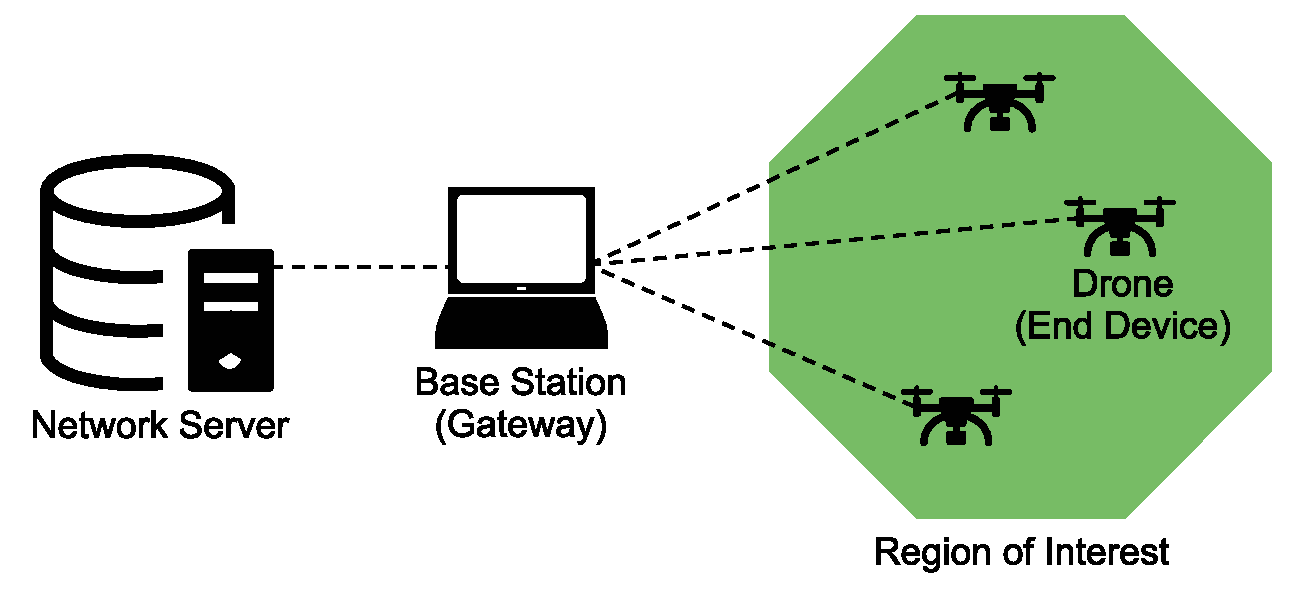
\includegraphics[width=0.7\linewidth]{figs/Jihwan/Network Diagram of LoRa.eps}
    \caption[LoRaWAN Network Diagram for Extra-UAV Communication]
    {\gls{lorawan} network diagram for extra-\gls{UAV} communication. More base stations, \gls{roi}s and drones can be connected to the network server as necessary.}
    \label{fig:euc_network_diagram}
\end{figure}

When generating the path plan of the drones in the mission planning framework (Section~\ref{sec:msp}), a network simulation will be conducted to ensure signal stability throughout the entire duration of the mission. If the drone paths travel too far from the base station for a stable extra-\gls{UAV} communication to be maintained, the operator will be warned and advised to install another base station at a suitable location. 
 
\subsubsection{Simulation using ns-3}

To simulate the stability of \gls{lorawan} during a mission, ns-3\footnote{\url{https://www.nsnam.org/}} discrete-event network simulator will be used. ns-3 is a free and open-source software (GNU GPLv2 license) which allows the developer to incorporate custom models to construct the simulation scenario. 

\paragraph{LoRaWAN Model} The model was created by \cite{magrin2017lora} to create \gls{lorawan} simulations by establishing connections between custom end devices, gateways and network servers. Currently, the model only supports class A end devices at 868\,MHz (\gls{ism} band for EU) so additional components will need to be developed for implementation. 

\paragraph{Mobility Model} The model enables nodes to have defined position and velocities on a Cartesian plane. The generated path plans of the drones can be input to accurately simulate the network performance at any part of the \gls{roi} during the mission. 


\newpage
\fancyhead[C]{Thomas Turner}
\section{Custom Hardware} \label{section:Custom Hardware}
\subsection{Introduction and Philosophy}
Due to the specific operating environment, custom hardware is required. This is because the device cannot safely carry out emergency landing procedures when a fault is detected due to the difficulty of retrieval. Furthermore, any crashes can damage the onboard imaging sensors. Lastly, there is significant opportunity cost of delaying mapping as the equipment and manpower involved in demining would be ineffective until retrieval and repair or replacement of the device. 
\paragraph{When to use custom components}
\gls{COTS} options should always be considered before any custom part due to the significant design and testing costs associated with custom parts. Furthermore, \gls{COTS} options will often have shorter lead times and will benefit from sourcing at greater scales. However, when there are specific design requirements not met in the current market custom components need to be used.
\paragraph{Objectives}
All hardware should be easy and quick to debug, it should support redundancy and it should be as modular as possible. Furthermore, they should also line up with our sustainability and inclusion objectives by ensuring all components are \gls{RoHS} compliant and, where applicable, should support those with disabilities. I will design core components demonstrating the design principles explored however, not all hardware components are considered and there is significant room for future work.

\input{Thomas/Custom_Hardware/PCBS}
\subsection{Design Considerations}\label{sub_section:tgt_design_considerations}

\subsubsection{Built for compliance}
\paragraph{Regulations}
Compliance to local laws is an important part of \gls{PCB} design, to operate in the European Union it would need to be CE compliant and for general use it should be up to IPC-2221 standards\footnote{\url{https://www-eng.lbl.gov/~shuman/NEXT/CURRENT_DESIGN/TP/MATERIALS/IPC-2221A(L).pdf}}. To ensure the design was up to IPC-2221 standards all spacings and widths of traces are compliant throughout the design. To ensure a smooth compliance process for CE it was ensured all components are \gls{RoHS} compliant and all solder is lead free. Furthermore, at all times the industry standard best practices as outlined in IPC-2221 standards were followed.
\paragraph{Process}
Compliance is often confirmed by 3rd party labs, TUV SUD offers UA DoC (EMC) which is required for products under 75 VDC in Ukraine with the CE as pre-requisite\footnote{\url{https://www.tuvsud.com/en-us/services/product-certification/ukraine-safety-certification}}. However, before being sent to external labs it should be internally tested for \gls{EMI}, thermal stability and vibration robustness with rapid prototyping to ensure minimal redesigns are needed.

\subsubsection{Trace Lengths}\label{sub_sub_section:tgt_trace_lengths}
\paragraph{Signal Integrity and Timing}
All traces have propagation delay that increases linearly with length meaning that the longer the trace, the longer the delay. Furthermore, noise increases due to impurities and crosstalk. Therefore, trace length is minimised in the design process. Therefore, in all custom designs the large footprint devices such as connectors are placed at the edges and the \gls{MCU} is placed centrally.
\paragraph{Length Matching}
In synchronous communication methods the clock signal must be in sync with the data transmission. This means that the lines should be as similar in length as possible so that they arrive at the same delay. The faster the communication rate the stricter this must become as the clock signal frequency is increased.
\paragraph{Effect of vias}
Vias allow for the transference of signals between planes which is necessary for routing signals. However, they should be avoided as they introduce extra impedance, noise and delay. Furthermore, for synchronous high speed signals they should be included in trace length considerations as the line with fewer vias should be tuned to have a longer length to achieve the same delay.
\paragraph{Utility Regions}
Components with similar functionalities should be restricted to specific regions, this is because it reduces trace length, prevents interference between high and low frequency signals and makes thermal management easier. These regions are shown in Figure \ref{fig:custom_hardware_overview} for the custom components.

\subsubsection{Circuit Protection}\label{sub_sub_section:tgt_circuit_protection}
\paragraph{\gls{ESD}}
\gls{ESD} occurs when there is a significant static charge built up in a ground operator or contacting surface that is then shorted in contact with the board causing a current transient and circuit damage. IEC 61000-4-2 level 4 is the highest IEC 61000-4-2 standard at 8 kV contact/15 kV\footnote{\url{https://www.ti.com/document-viewer/lit/html/SSZT871}} and will be considered a lower bound specification for the design. 
\paragraph{Touch Protection Devices}
In order to protect against \gls{ESD} the circuit must provide a low resistance pathway to the ground. This can be using \gls{TVS} diodes that above certain voltages act like a wire that diverts the current flow\footnote{\url{https://resources.altium.com/p/pcb-design-guidelines-using-tvs-diode-transient-protection}}. In my designs I use the \gls{TVS} diode produced by Vishay (Part number: VCUT03G1-SD0) bidirectional \gls{TVS} diode that are rated to 30kV in both contact and air gap\footnote{\url{https://www.vishay.com/docs/86315/vcut03g1-sd0.pdf}} to ensure to \gls{ESD} protection. 
\paragraph{Over current protection}
Series resistors are the best way to protect a device against transient current spikes as they mitigate the peak current. Therefore, for serial debugging terminals I ensured that all connections have 100$\ohm$ series resistors in case of accidental short circuits by the user, this is only appropriate in signal traces however, as otherwise the power dissipation in normal operation is too high. Therefore, 2.6A fuses are used in the power lines of both modules to protect against short circuits, I selected a resettable manufactured by Bourns (Part number: MF-LSMF260/6X-2) in order to ensure it can be repaired easily in the field. Both these measures are in line with IPC-2221 standards.
\paragraph{Placement}
Protections should be as close to possible sources so the least number of components and wires get damaged in failure. Therefore, all \gls{TVS} diodes are placed near touched areas or interfaces, series resistors are placed as close as possible to prevent wire transients and fuses are placed before the power is connected to the power and ground planes. This minimises the damage potential.

\subsubsection{Trace Widths and Spacing}\label{sub_sub_section:tgt_trace_width}
\paragraph{Impedance Control}
The copper thickness is a key metric in the cost of a \gls{PCB} as the material cost is the most significant cost and manufacturers typically have fixed options. The thinnest standard option offered by PCBway is 1 Oz/foot$^2$ foot of copper and therefore I used this throughout my designs. To control the impedance of a trace calculated trace widths using the industry standard IPC-2221 compliance formula\footnote{\url{https://resources.altium.com/p/ipc-2221-calculator-pcb-trace-current-and-heating}} to ensure it is compliant with industry standard practices. Setting the expectable temperature rise to 10\degree C and thickness to 1 Oz/foot$^2$, a trace of width 12 mil (0.3048mm) is rated up to 1A and a trace width of 6 mil (0.1528mm) is rated at over 0.6A. Given that traces below 6 mil incur extra manufacturing cost\footnote{\url{https://www.pcbway.com/pcb_prototype/PCB_Design_Rule_Check.html}} for signals 6 mil traces are used and for power-carrying traces 12 mil traces are used.
\paragraph{Crosstalk}
When traces are too close too each other they can induce signals in each other, this causes inaccuracies that can cause Analogue to Digital converter to have bit errors\footnote{\url{https://resources.altium.com/p/crosstalk-basics-pcb-design?}}. Therefore, the Radio Frequency input for the \gls{GNSS} module is kept away from all other components and the ground and voltage planes as shown in Figure \ref{fig:gnss_render}) to ensure that there is no mutual inductance. This ensures that the designs reduce the effect of \gls{EMI} in line with IPC-2221 standards and CE certification.

\subsubsection{Layers}\label{sub_sub_section:tgt_layers}
\paragraph{Two Layers}
The simplest and most cost effective option in \gls{PCB} design is two copper layers separated by a dielectric. By using a copper filled regions you can create a ground plane and a power plane that effectively distribute charge and maintain voltage integrity. The simplicity of the \gls{GNSS} module means that two layers is the best option. This comes at the cost of more difficult component placement and a slightly less stable power and ground plane. To mitigate the instability, distributed ceramic capacitors between the planes that filter high frequency noise in voltage levels, maintaining integrity. These capacitors are best placed next to sensors and processers to ensure stable, low noise readings. .
\paragraph{Four or More Layers}
When circuits become more complex, a purpose ground and power plane in between the top and bottom plane can allow for greater packing density of components. It also mitigates the effect of \gls{EMI} as dedicated planes have a lower impedance. This means that for complex designs with many sensors, like the flight controller module, four layer \gls{PCB}s are the best option. Furthermore, if the complexity of the design is greater you can add further ground and power planes for analogue signals, high frequency signals or for regular signals to support greater component density and \gls{EMI} reduction. For the flight controller I used signal-ground-power-signal layers to minimise loop inductance.

\subsection{Debugging and Interfaces}\label{sub_sub_section:debugging}
\paragraph{Technical Debugging}
There easy to use male pin headers in both designs shown in Figure \ref{fig:custom_hardware_overview} so that a \gls{SWD} debugger can be connected, furthermore, for signalling debugging the detachable ports for the \gls{CAN} bus mean a debugging computer can simply connect. This is so technically skilled operators can inspect system level signals and specific board operations.
\paragraph{Field Debugging}
The use of technical debugging experts should always be avoided if possible to reduce capital expenditure and delay. Therefore the custom flight controller has a simple 4 \gls{LED} array for basic error codes that can isolate the problem so it can be fixed or so that only a specific, replaceable component, can be sent for repair and switched out with a backup. These codes are shown in Table \ref{tab:error_codes} where the colours are the \gls{LED}s and the x denotes blinking, the null state is a solid green \gls{LED} only.  The inclusion of the green LED has three key purposes: firstly, it blinks to denote between modules, secondly it gives clear visualisation that no tests have failed and lastly it ensures the codes are red in the right order no matter the orientation. It is also a different brightness to the red \gls{LED}s allowing for use by colour-blind operators in line with the inclusion objectives of the project.
\begin{table}
\begin{tabular}{|l|c|l|c|l|c|l|c|}
\hline
\textbf{Failure} & \textbf{Code} & \textbf{Failure} & \textbf{Code}& \textbf{Failure} & \textbf{Code} & \textbf{Failure} & \textbf{Code} \\
\hline
CAN 1 & \drawcode{white}{red}{red}{red} & CAN 2 & \drawcode{blinkgreen}{red}{red}{red} &
GNSS 1 & \drawcode{white}{red}{red}{white} & GNSS 2 & \drawcode{blinkgreen}{red}{red}{white}\\

Flight Controller & \drawcode{white}{red}{white}{white} & BMS & \drawcode{blinkgreen}{red}{white}{white} &
Collision 1 & \drawcode{white}{white}{red}{white} & Collision 2 & \drawcode{blinkgreen}{white}{red}{white}\\

ESC 1 & \drawcode{white}{blinkred}{blinkred}{blinkred} & ESC 2 & \drawcode{white}{red}{blinkred}{blinkred} &
ESC 3 & \drawcode{white}{red}{red}{blinkred} & ESC 4 & \drawcode{white}{red}{blinkred}{red}\\

Altimetry 1 & \drawcode{white}{white}{white}{red} & Altimetry 2 & \drawcode{blinkgreen}{white}{white}{red} &
LoRA & \drawcode{white}{white}{red}{red} & Unknown & \drawcode{blinkgreen}{blinkred}{blinkred}{blinkred}\\
\hline
\end{tabular}
\caption{Flight Controller LED Error Codes}
\label{tab:error_codes}
\end{table}
\paragraph{Post Failure Analysis}
If there is a crash that causes significant damage, and due to the volatile nature of \gls{RAM} memory, some failures cannot be detected directly with the device. Therefore, the flight controller has a removable microSD card to record flight data. In addition, the backup power supply, as seen in Figure \ref{fig:custom_hardware_overview}, provides enough power that even in complete failure it can write the final few error messages. Therefore, this can be retrieved, downloaded and sent for analysis quickly to find the source of failure.
\paragraph{Interfaces}
It is important that all interfaces between modules are easy to access, protected and consistent. For both designs screw-in connectors are used for the battery supply to ensure a strong power connection whilst also being removable. For all communication signals a 3 pin JST connector with locking ensuring any disconnections due to vibrations are minimised. For the \gls{CAN} signals the third pin is used as a shared ground so the signals do not drift between boards and all have a shared ground level. Lastly, for the debugging interface male Dupont header is used so that the user can attach wires easily. All interfaces are protected with \gls{TVS} diodes to ensure no accidental \gls{ESD} events when connecting or disconnecting.


\begin{comment}
\subsubsection{Component Placement}\label{sub_sub_section:tgt_component_placement}

\paragraph{Thermal Considerations}
Heat dissipating elements, typically diodes and resistors, can cause damage to electronic component, therefore, heat sinks or controlled airflows are sometimes required. This consideration is why on my devices Buck Converters of above 90\% are used instead of the less efficient \gls{LDO} which would have an efficiency of 66\% when converting from 5V to 3.3V. This, in addition to the low power draws of all other components, means that no explicit thermal management is needed.
\end{comment}
\subsection{Custom Components}\label{sub_sub_section:tgt_custom_components}

\subsubsection{Component Selection}\label{sub_sub_section:tgt_component_selection}
\begin{table}[htbp]
  \centering
  \begin{tabular}{|l|c|c|c|c|}
    \hline
    \textbf{Name} & \textbf{Price} & \textbf{Gyro Noise} & \textbf{Accel Noise} & \textbf{Gyro Freq.} \\
    & £ & (mdps/$\sqrt{\text{Hz}}$) & (µg/$\sqrt{\text{Hz}}$) & (kHz) \\
    \hline
    ICM-42688-P\tablefootnote{\url{https://invensense.tdk.com/products/motion-tracking/6-axis/icm-42688-p/}} & 329 & 2.8 & 70 & 32 \\
    MPU-6500\tablefootnote{\url{https://invensense.tdk.com/products/motion-tracking/6-axis/mpu-6500/}}    & 423 & 10  & 300 & 32 \\
    BMI323\tablefootnote{\url{https://www.bosch-sensortec.com/products/motion-sensors/imus/bmi323}}      & 157 & 7   & 180 & 12.5 \\
    \hline
  \end{tabular}
  \caption{Comparison of Selected IMUs}
  \label{tab:imu-comparison}
\end{table}

\begin{table}[htbp]
  \centering
  \begin{tabular}{|l|r|r|r|r|r|r|}
    \hline
    \textbf{Name} & \textbf{Flash (KB)} & \textbf{RAM (KB)} & \textbf{Clock (MHz)} & \textbf{Price (£)} & \textbf{CAN} & \textbf{Pins} \\
    \hline
    MSPM0G3506SRHBR\tablefootnote{\url{https://www.ti.com/product/MSPM0G3506/part-details/MSPM0G3506SRHBR}} & 32 & 32 & 80 & 87 & 1 & 32 \\
    STM32H743VGT6\tablefootnote{\url{https://www.st.com/en/microcontrollers-microprocessors/stm32h743vg.html}} & 1000 & 1000 & 480 & 737.21 & 2 & 100 \\
    STM32F765VGT7\tablefootnote{\url{https://www.st.com/en/microcontrollers-microprocessors/stm32f765vg.html}} & 1000 & 512 & 216 & 812 & 3 & 100 \\
    \hline
  \end{tabular}
  \caption{Comparison of MCUs}
  \label{tab:mcu-comparison}
\end{table}

\begin{table}[htbp]
  \centering
  \begin{tabular}{|l|c|c|c|c|c|}
    \hline
    \textbf{Name} & \textbf{Price (£)} & \textbf{RTK} & \textbf{Update Rate (Hz)} & \textbf{Dead Reckoning} & \textbf{Precision (m)} \\
    \hline
    MAX-F10S-00B\tablefootnote{\url{https://www.u-blox.com/en/product/max-f10s-module}} & 1109 & No  & 10 & No  & 1    \\
    ZED-F9P-05B\tablefootnote{\url{https://www.u-blox.com/en/product/zed-f9p-module}}    & 9082 & Yes & 5  & No  & 0.01 \\
    LC29HEAMD\tablefootnote{\url{https://www.quectel.com/product/gnss-lc29h/}}         & 4091 & Yes & 10 & No  & 0.01 \\
    LC29HAAMD\tablefootnote{\url{https://www.quectel.com/product/gnss-lc29h/}}         & 769  & No  & 10 & No  & 1    \\
    LG69T-AP\tablefootnote{\url{https://www.quectel.com/product/gnss-lg69t-series/}}   & 5877 & Yes & 10 & Yes & 0.01 \\
    \hline
  \end{tabular}
  \caption{Comparison of GNSS Modules}
  \label{tab:gnss-modules}
\end{table}

\paragraph{\gls{IMU}}
While the BMI323 is cheaper it has higher noise characteristics than the the ICM-42688-P, therefore the latter was selected for use on all boards due to its low price point and high performance. The use of the same \gls{IMU} over all modules should be maintained if possible so that the control characteristics are unchanged across devices and lower costs due to higher order quantities.
\paragraph{\gls{MCU}}
For the flight controller the STM32H743VGT6 is the best option given its \gls{RAM}, price point and support of dual \gls{CAN} buses. However, for the less computationally intense operations required for the \gls{GNSS} module the smaller footprint (due to the lower number of pins) and lower priced MSPM0G3506SRHBR is a better option.
\paragraph{\gls{GNSS} Module}
Exact positions for where the images were taken to centimetre precision is required as discussed in Section \ref{GPR_design}, this is possible using a \gls{RTK} setup with a base station sending out correction vectors over LoRa getting within centimetre accuracy\cite{RTK_LORA}. Furthermore, in the case of the loss of all \gls{GNSS} signal built in dead reckoning, allowing \gls{RTS}, is also a desirable feature. Therefore, the LG69T-AP is selected. However, when not executing imaging tasks, this precision is not needed and the modules are more expensive than the \gls{GNSS} modules without these features. Therefore, for the redundant device the MAX-F10S-00B was selected, and is shown in \ref{fig:custom_hardware_overview}, due to the significantly better documentation available and similar price points when compared to the LC29HAAMD.

\subsubsection{Power Supply}\label{sub_sub_section:tgt_power_supply}
\begin{table}[htbp]
  \centering
  \begin{tabular}{|l|r|r|r|}
    \hline
    \textbf{Component} & \textbf{Flight Controller} & \textbf{Redundant GNSS} & \textbf{Value}\\
    \textbf{} & \textbf{Quantity} & \textbf{Quantity} & \textbf{(mA)}\\ 
    \hline
    ICM-42688-P\tablefootnote{\url{https://invensense.tdk.com/products/motion-tracking/6-axis/icm-42688-p/}} & 2  & 1 & 0.88\\
    STM32H743VGT6\tablefootnote{\url{https://www.st.com/en/microcontrollers-microprocessors/stm32h743vg.html}} & 1 & 0 & 165\\
    MSPM0G3506SRHBR\tablefootnote{\url{https://www.ti.com/product/MSPM0G3506/part-details/MSPM0G3506SRHBR}} & 0 & 1 & 8\\
    MAX-F10S-00B\tablefootnote{\url{https://www.u-blox.com/en/product/max-f10s-module}} & 0 & 1 & 200\\
    LEDs & 3 & 0 & 20 \\
    Misc & 1 & 1 & 20 \\ 
    \hline
    \textbf{Total} & \textbf{246.76 mA} & \textbf{228.88 mA} & \textbf{}\\
    \hline
  \end{tabular}
  \caption{Current Draws}
  \label{tab:current-draws}
\end{table}
\paragraph{Main Power Supply}
In both the GNSS module and the flight controller module the same power setup was used, created in Webench Power Designer\footnote{\url{https://webench.ti.com/power-designer/switching-regulator}}. The key decision metrics were efficiency and cost.  Efficiency is of high importance due to the thermal management on the board. The design selected has over 90\% efficiency \ref{fig:power_graphs} throughout the expected operating current window. As shown in the schematic \ref{fig:power_supply_schematic} there is a fuse to protect from short circuits and a \gls{TVS} diode to protect against \gls{ESD} that someone connecting the power might cause. There are also capacitors of 22uF and 4.7uF to provide current during spikes and smooth the power supply current.
\begin{figure}[ht]
  \centering
  \includegraphics[width=\textwidth]{figs/Thomas/Custom Hardware/Power Supply.png}
  \caption{KiCad Power Supply Schematic}
  \label{fig:power_supply_schematic}
\end{figure}



\begin{figure}[ht]
 \centering
 \begin{minipage}[t]{0.48\textwidth}
  \centering
  \includegraphics[width=\textwidth]{figs/Thomas/Custom Hardware/charging_curve.png}
  \caption{Backup Power Supply Charging Curve}
  \label{fig:charging_curve}
 \end{minipage}
 \hfill
 \begin{minipage}[t]{0.48\textwidth}
  \centering
  \includegraphics[width=\textwidth]{figs/Thomas/Custom Hardware/charging_curve.png}
  \caption{Backup Power Supply Price Curve}
  \label{fig:price_curve}
 \end{minipage}
\end{figure}



\begin{comment}
      \hfill
  \begin{subfigure}[b]{0.6\textwidth}
    \includegraphics[width=\textwidth]{figs/Thomas/Custom Hardware/Power Module Effciency.png}
    \caption{Power Module Efficiency}
    \label{fig:power_efficiency}
  \end{subfigure}
  \caption{Custom Power Supply}
  \label{fig:power_graphs}
\end{comment}
\paragraph{Backup Power Supply}
The telemetry recordings of the flight controller are vital for crash analysis. However, in cases of sudden electrical failure the data recording will stop before writing the final state vectors and error codes. For example, if before a short circuit the current draw from an \gls{ESC} starts spiking that message needs to be recorded even if a fuse immediately burns shutting down the power supply. Therefore, a supercapacitor in series with a drain resistor is used \ref{fig:power_supply_schematic}. The capacitor selected is rated up to 5.4V at 0.47F\footnote{\url{https://uk.rs-online.com/web/p/supercapacitors/2506967}}. 
\begin{equation}
t = \frac{C \cdot (V_0 - V_{\text{cutoff}})}{I}
\label{eq:discharge_time}
\end{equation}
\begin{equation}
t_{\text{worst-case}} = \frac{0.47 \cdot (3.3 - 2.8)}{1} = 0.235\ \text{seconds}
\label{eq:worst_case_time}
\end{equation}
\begin{equation}
\tau = R \cdot C = 20 \cdot 0.47 = 9.4\ \text{seconds}
\label{eq:charging_time_constant}
\end{equation}
The time before dropout, with the worst case conditions is over 0.2 seconds \ref{eq:worst_case_time}, this will provide sufficient time to record any last messages. Furthermore, the time constant is 9.4s \ref{eq:charging_time_constant} meaning that there are current spikes when turning the device on but it is still charged over 3V within 30 seconds \ref{fig:charging_curve}.

\subsubsection{Comparison to Commercial Options}\label{sub_sub_section:tgt_commercial_options}
\begin{table}[htbp]
  \centering
  \begin{tabular}{lrr}
    \toprule
    \textbf{Category}         & \textbf{Redundant GNSS Cost} & \textbf{Flight Controller Cost}\\ 
    \midrule
    Passive Components        & £140.40  & £385.00\\
    Active Components         & £1699.10 & £1865.10\\
    Headers/Connectors        & £179.50  & £278.40\\
    PCB \& Assembly           & £262.14  & £334.04\\
    \midrule
    \textbf{Total}            & £2281.14 & £2862.54\\
    \bottomrule
  \end{tabular}
  \caption{Cost of custom component (100 units)}
  \label{tab:aggregated-cost}
\end{table}


The CUAV X7+\footnote{\url{https://store.cuav.net/shop/x7/}} GPS compatible option costs £339.75 per unit and provides the same core functionality as the custom flight controller including dual \gls{CAN} ports. This can be combined with the flight controller compatible with the CUAV C-RTK 9Ps Positioning Module\footnote{\url{https://store.cuav.net/shop/c-rtk-9ps/}} that costs £332.91 for a drone-base station pair and provides \gls{RTK} \gls{GNSS}. This is a significant increase in cost however, it would not require development and may be a superior option in the testing phase. However, for deployment the custom components should be used given the cost implications and that the custom \gls{GNSS} module is fully control capable and the commercial option is not. 

%%%%
% \newacronym{LIPO}{LIPO}{lithium polymer}
% \newacronym{LIION}{Li-ion}{lithium-ion}
% \newacronym{gbp}{GBP}{Great British Pound}
% \newacronym{RESC}{RESC}{resonant switched capacitor}
% \newacronym{6s}{6s}{6-cell series}
% \newacronym{6s3p}{6s3p}{6-series 3-parallel}
% \newacronym{tim}{TIMS}{thermal interface materials}
% \newacronym{DCDC}{DC-DC}{Direct Current to Direct Current [power converter]
% }

% \newacronym{BS}{BS}{British Standards}
% \newacronym{ESR}{ESR}{equivalent series resistance}
% \newacronym{I2C}{I\textsuperscript{2}C}{Inter-Integrated Circuit }
% \newacronym{UART}{UART}{Universal Asynchronous Receiver/Transmitter }
% \newacronym{SRAM}{SRAM}{static random-access memory}
% \newacronym{SOC}{SOC}{state of charge}
% \newacronym{NTC}{NTC}{negative-temperature-coefficient}
% \newacronym{EKF}{EKF}{extended Kalman filter}
% \newacronym{FEM}{FEM}{finite element method}
% \newacronym{MOSFET}{MOSFET}{metal–oxide–semiconductor field-effect transistor}
%%%%

\fancyhead[C]{Samuel Grace}

\section{Battery Management System and Battery Hardware}
\label{sec:bms}
\subsection{Introduction and Motivation}

Although most drones do not contain one, an inbuilt \gls{BMS} \cite{SON2023120186} provides many key advantages when performing landmine detection. A \acrshort{BMS}, along with the corresponding bespoke circuit topology, supports the complex control system, high-quality sensor requirements and extended mission duration capabilities necessary for effective landmine detection. Additionally, it is possible to program a \acrshort{BMS} to optimise the battery cells’ lifespan; both reducing the operating cost and the environmental impact of the drone.

\subsection{Design and Component Selection}

Optimal design of the \acrshort{BMS} and the selection of appropriate components will determine the eventual success of the drone. It is necessary to choose components that will achieve the desired design solution, while balancing the considerations of cost, availability and sustainability.


\subsubsection{Cell Comparison and Selection}

The most important decision is selecting a battery cell chemistry. Drones typically use \gls{LIPO} batteries\footnote{\acrshort{LIPO} batteries are a subset of \acrshort{LIION} batteries. Conventionally, \acrshort{LIION} cells are taken to be those with a liquid electrolyte, whereas \acrshort{LIPO} cells have a polymer electrolyte.} due to their high maximum discharge current \cite{10808488}. However, following recent developments, \gls{LIION} batteries now have approximately 30\% higher gravimetric energy density than \acrshort{LIPO} cells  \cite{Agrawal_2008}. Higher energy density permits longer flight times and carrying more sophisticated sensors, improving both the quality and quantity of the data gathered. \acrshort{LIION} cells are also more durable and safer than \acrshort{LIPO} cells, as they are more thermally stable and have a more rigid internal structure \cite{bergveld2014battery}. The decision matrix shown in Table \ref{tab:battery_comparison} compares different components based on set criteria to select the specific type of \acrshort{LIION} cell. The process involves weighting different factors according to their relative importance. The total energy of the cell is the most important factor, as it is directly proportional to the flight time and affects how much power is available for sensing. Weight is the next most significant factor since it affects both flight time and stability. Cost is the least important factor because the price of the cells is low compared to the price of other components of the drone. The scores for each factor are calculated by normalising relative to the \textit{best} of the three values and multiplying the normalised score by 10. The \textit{best} energy value is the highest, whereas the \textit{best} weight and the \textit{best} price values are the lowest. 

\begin{table}[h!]
\centering
\begin{tabular}{|l|c|c|c|c|}
\hline
\textbf{Specification} & 
\makecell{\textbf{Samsung}\\\textbf{3500mAh}\\\textbf{18650 Li-ion Cell}} &
\makecell{\textbf{Panasonic}\\\textbf{2040mAh}\\\textbf{18500NCR Li-ion Cell}} & 
\makecell{\textbf{Overlander}\\\textbf{4500mAh}\\\textbf{21700 Li-ion Cell}} & 
\textbf{Weighting} \\
\hline
\textbf{Energy (Wh)} & 12.95 & 7.55 & 16.65 & 60\%\\
\textbf{Energy Score} & 7.8& 4.5& 10.0& - \\\hline
\textbf{Weight (g)} & 48.5 & 33 & 70 & 30\% \\
\textbf{Weight Score} & 6.8& 10.0& 4.7& - \\
\hline
\textbf{Price \acrshort{GBP}} & 6.98 & 8.99 & 9.98& 10\%\\
\textbf{Price Score} & 10& 7.8& 7.0& - \\
\hline
\textbf{Total Score} & 7.7& 6.5& 8.1& 100\% \\
\hline
\end{tabular}
\caption[Battery Cell Comparison]{Comparison for energy capacity, weight, and price, with normalised scores and weighted totals.}
\label{tab:battery_comparison}
\end{table}

The \textbf{total score} \( S \) is calculated using Equation \ref{eq:score_formula}; all values used are taken from Overlander Batteries.\footnote{Overlander Batteries: \url{https://www.overlander.co.uk/}}

\begin{equation} \label{eq:score_formula}
S = w_C \times 10 \times\frac{\text{Energy}}{\text{Max. Energy}} + w_W \times 10 \times\frac{\text{Min. Weight}}{\text{Weight}} + w_P \times 10 \times\frac{\text{Min. Price}}{\text{Price}}
\end{equation}
\[(
\text{where }w_C, w_W, w_P \text{ are the importance weightings for capacity, weight and price respectively})
\]

From the results shown in Table \ref{tab:battery_comparison}, the design decision taken was to select the \textbf{Overlander 4500mAh 21700 Li-ion Cell}. Using \acrshort{LIION} cells improves reliability significantly because \acrshort{LIION} cells are much more durable than \acrshort{LIPO} cells due to their more rigid metal casing. Also, \acrshort{LIION} cells are less prone to thermal runaway, which reduces the risk of catastrophic failure when operating in hot, arid climates. Furthermore, \acrshort{LIION} cells are more environmentally sustainable than \acrshort{LIPO} cells because they have a longer average lifetime and higher recyclability.

However, there are important sustainability considerations regarding the \acrshort{LIION} cells, such as the vast quantities of energy required in the production process \cite{environments12010024}. It is also important to ensure that the lithium mining process used to source the material for the battery is conducted in both an environmentally and ethically sustainable way \cite{EnergyFuturesLab_2022}. 

\textbf{Overlander}, the chosen supplier for the batteries, has detailed policies about their compliance in all of these areas, which guarantees that the cells used are sustainable. The custom design of the \gls{BMS} ensures that cell balancing, charging and discharging strategies are optimised to maximise battery life and durability. This optimisation further improves the sustainability by reducing the frequency at which the \acrshort{LIION} cells must be replaced. 

\subsubsection{Microcontroller, Charger and Sensor Selection}
\label{microcon}

The \acrshort{BMS} requires a microcontroller with sufficient processing power to perform the state estimations using Kalman filters and to run the algorithms controlling the battery cells. The device used must also be able to communicate with sensors and other devices using \gls{I2C} and \gls{UART} protocols \cite{Denggao2022}. Accordingly, the \textbf{STM32F405} microcontroller was selected. It offers a clock speed of 168 MHz, 192 Kbytes of \gls{SRAM} and 512 Kbytes of flash memory \cite{st_dm00037051}. These performance metrics mean that the \textbf{STM32F405} is sufficiently powerful to compute accurately the state estimations and run the \acrshort{BMS} algorithms. \textbf{iMAX B6 V2 Chargers} were selected, allowing for quick and efficient charging between missions \cite{digikey_prt16793}.

A variety of measurements are required to provide the \acrshort{BMS} with the required data to estimate the \gls{SOC} of the cells. First, the \textbf{TI BQ76972} sensors provide accurate cell voltage measurements and communicate using the \acrshort{I2C} interface. The \textbf{TI BQ769142} battery monitor provides measurements of the battery current, and also communicates using the \acrshort{I2C} protocol. An advantage of using the \textbf{TI BQ769142} is that it additionally supports temperature sensing using \gls{NTC} thermistors positioned inside the battery pack; the thermistors are used to provide accurate measurements for each cell within the battery cell stack. Texas Instruments provided the methodology that was followed \cite{TI_SNIA032}, specifically for use within a \gls{BMS}.

\subsubsection{Kalman Filtering Techniques}
\label{kalm}

Kalman filters are implemented on the \textbf{STM32F405} microcontroller to estimate the various states in the battery, such as temperatures, voltages and currents. The Kalman filter's purpose is to estimate the states using indirect, uncertain measurements \cite{kalfilt}. 

For each state, the underlying physical process is modelled in state-space form, and the system is discretised to allow a Kalman filter to be implemented in C using a Kalman filtering library designed for embedded systems \cite{computers11110165}. As an example of the process, the estimation of the \gls{SOC} using an \gls{EKF} was simulated. The \gls{EKF} algorithm is explained in detail by \cite{kalfilt}.  The \gls{SOC} is defined by Equation \ref{eq:soc}, where $C$ represents the battery's capacity.

\begin{equation}
\label{eq:soc}
\text{SOC (\%)} = 100 \times \frac{C_{\text{releasable}}}{C_{\text{rated}}}
\end{equation}

For the \gls{SOC} measurement, an \gls{EKF} is used in conjunction with the Coulomb counting method to estimate the \gls{SOC}. The \gls{EKF} was chosen over other methods, such as using a particle filter, since the \gls{EKF} is significantly less computationally intensive when working with few states, as is the case here \cite{STELZER20171483}. The \gls{EKF} accounts for measurement noise, which allows the \gls{EKF} to produce a high-fidelity estimate of the \gls{SOC} variation \cite{Zaki2025}.

 The simulation for the \gls{SOC} estimation process was performed using the Simscape Battery Toolbox, by adapting an existing model template.\footnote{\url{https://mathworks.com/help/simscape-battery/ug/estimate-battery-soc-using-kalman-filter-example.html}} The results are shown in Figure \ref{fig:bmsestimefk}, with Figure \ref{fig:coolomb} showing the estimate produced solely using the state-space model of the process. The residual error is clearly visible when relying solely on the state-space model, which suggests that a more sophisticated approach is required. Figure \ref{fig:kalmeff} shows the results of applying the \gls{EKF}, which successfully removes the offset that is visible in Figure \ref{fig:coolomb}.


\begin{figure}[H]
    \centering
    \begin{subfigure}[b]{0.49\textwidth} % Use [b] to align captions at the bottom
        \centering
        \includegraphics[width=\textwidth]{figs/Samuel/Figures/plotsbattest (1) (cropped) (pdfresizer.com).pdf}
        \caption{Estimate using Coulomb counting.}
        \label{fig:coolomb}
    \end{subfigure}
    \hspace{0\textwidth}
    \begin{subfigure}[b]{0.49\textwidth} % Use [b] to align captions at the bottom
        \centering
        \includegraphics[width=\textwidth]{figs/Samuel/Figures/plotsbattest (1) (cropped) (pdfresizer.com) (1).pdf}
        \caption{Estimate additionally using \gls{EKF}.}
        \label{fig:kalmeff}
    \end{subfigure}
    \caption[Comparison of State of Charge Estimates]{Comparison of State of Charge estimates using the Simscape Kalman Filter Template}
    \label{fig:bmsestimefk}
\end{figure}

\subsection{Internal System}

The overall structure of the \acrshort{BMS} is shown in Figure \ref{fig:bms_layout}, adapted from \cite{7555475}. For clarity, the battery pack depicts one set of the \acrshort{6S} cells. In reality, the system has a \acrshort{6S3P} configuration of cells. Sensor information from each cell in the battery pack is transmitted to the State Estimator, where Kalman filtering techniques are used to infer the states from the measurements. The State Estimator, including the \gls{EKF}, was incorporated into the model in MATLAB and Simulink utilising the Simscape Battery Toolbox.

The Master Control Unit represents the \textbf{STM32F405} microcontroller chosen in Section \ref{microcon}. The microcontroller implements the \gls{RESC} switching techniques detailed in Section \ref{swit}, as depicted by the \textbf{Cell Equalisation} component of the BMS.

\begin{figure}[H]
  \centering
  \vspace{5mm}
  \includegraphics[width=0.75\textwidth]{figs/Samuel/Figures/BMS Internal (1)-cropped.pdf}
  \caption[Battery Management System Layout]{Battery Management System Layout adapted from \cite{7555475}}
  \label{fig:bms_layout}
  \vspace{5mm}
\end{figure}






\subsubsection{Battery Cell Stack Configuration}

A simplified diagram of the cell switching layout used is shown in Figure \ref{fig:bcs}. The switching topology used is the \gls{RESC} layout. For conciseness, Figure \ref{fig:bcs} shows a simplified \gls{6S} circuit. In reality, a \gls{6S3P} layout is used, but this change does not affect the principles of operation. 

The use of capacitors, inductors and resistors allows for reduced equalisation time and less energy loss compared to simpler switched-capacitor methods \cite{8467638}. The core ideas and theory used to develop the \gls{RESC} layout shown in Figure \ref{fig:bcs} are discussed in \cite{8681672}, and additional simulation and modelling are utilised to verify the configuration's applicability in this context.

\begin{figure}[H]
\centering
\vspace{10mm}
\includegraphics[width=0.99\textwidth]{figs/Samuel/Figures/resc1-cropped.pdf}
\caption[Simplified Battery Cell Stack Configuration]{Simplified battery cell stack configuration, adapted from \cite{8467638}}
\label{fig:bcs}
\end{figure}

\subsubsection{Cell Switching Simulations}
\label{swit}

The \gls{RESC} switching technique outlined in \cite{8467638} was implemented in MATLAB, and the results obtained are shown in Figure \ref{fig:resccrop}. The methodology involved initialising each battery voltage with a random value between 3 V and 4 V and then performing the equalisation strategy. Figure \ref{fig:reccrop} shows the results obtained when using a simpler switched capacitor equalisation strategy. By contrasting the two plots shown in Figure \ref{fig:rescvrec}, the improved equalisation time given by the \gls{RESC} strategy can be observed. 

The results produced by the simulation are consistent with results from similar models \cite{8467638}, albeit for cells with significantly different parameters. The moderate differences in cell voltages model a situation where a cell is damaged or unusable, and due to the cell stack configuration, normal operation can be quickly resumed by equalising the remaining cells.

\begin{figure}[H]
    \centering
    \vspace{5mm}
    \begin{subfigure}[b]{0.4\textwidth} % Use [b] to align captions at the bottom
        \centering
        \includegraphics[width=\textwidth]{figs/Samuel/Figures/cellV-cropped.pdf}
        \caption{\gls{RESC} switching strategy}
        \label{fig:resccrop}
    \end{subfigure}
    \hspace{0.07\textwidth}
    \begin{subfigure}[b]{0.388\textwidth} % Use [b] to align captions at the bottom
        \centering
        \includegraphics[width=\textwidth]{figs/Samuel/Figures/recpdf-cropped.pdf}
        \caption{Simpler switched-capacitor strategy}
        \label{fig:reccrop}
    \end{subfigure}
    \caption[Comparison of Cell Equalisation Strategies]{Comparison of cell equalisation strategies using the method outlined in \cite{8467638}}
    \label{fig:rescvrec}
\end{figure}

\subsubsection{Thermal Management Design and Simulations}

Designing an efficient thermal management system has numerous advantages for battery operation, with the most significant benefit being the ability to extend the cells' lifetimes by 30-50\% \cite{TOGUN20251077}. The design used in this \gls{BMS} focuses on utilising passive cooling techniques to regulate and balance the battery's temperature. Specifically, \gls{TIMS} are used to regulate the transfer of heat between individual cells and their surroundings. In this design, a thin thermally conductive layer is inserted between the cells to aid heat dissipation. This passive cooling measure is especially useful when there are many cells, ensuring that even if some cells generate more heat, the overall temperature distribution remains balanced. Figure \ref{fig:tempythings} shows how temperature influences the discharge time (Figure \ref{fig:tempy1} from Chen, 2013 \cite{chen2013heat}) and the cycle life (Figure \ref{fig:tempy2} from \cite{REZVANIZANIANI2014110}). These graphs illustrate the importance of effective thermal management. Maintaining an operating temperature within the 20$^\circ\text{C}$ to 45$^\circ\text{C}$ range prevents the cell from discharging too rapidly and maximises the cycle life.

\begin{figure}[H]
    \centering
    \begin{subfigure}[b]{0.47\textwidth} % Use [b] to align captions at the bottom
        \centering
        \includegraphics[width=\textwidth]{figs/Samuel/Figures/chenbattery.png}
        \caption{Cell discharge curves for varying temperatures \cite{chen2013heat}}
        \label{fig:tempy1}
    \end{subfigure}
    \hspace{0.04\textwidth}
    \begin{subfigure}[b]{0.47
    \textwidth} % Use [b] to align captions at the bottom
        \centering
        \includegraphics[width=\textwidth]{figs/Samuel/Figures/Lithium-ion-battery-life-vs-temperature-and-charging-rate-36-39-44-45.png}
        \caption{Variation of cycle life vs. temperature \cite{REZVANIZANIANI2014110}}
        \label{fig:tempy2}
    \end{subfigure}
    \caption[Effects of Temperature Variation on Cell Properties]{Effects of temperature variation on cell properties, figures from \cite{chen2013heat} (a) and \cite{REZVANIZANIANI2014110} (b).}
    \label{fig:tempythings}
\end{figure}

Using the Simulink and Simscape software, a high-fidelity model of the cells with the passive thermal management system was constructed. Cooling analysis of the battery was performed using simulation data, allowing for the use of realistic heat fluxes. The cell geometries were modelled, and the \gls{FEM} was utilised to analyse the heat evolution over time by adapting an existing Simulink template.\footnote{\hyperlink{https://mathworks.com/help/pde/ug/battery-module-cooling-analysis-and-reduced-order-thermal-model.html}{mathworks.com/help/pde/ug/battery-module-cooling-analysis-and-reduced-order-thermal-model.html}} To provide meaningful results, the thermal analysis was run in parallel with the simulation example performed in Section \ref{mocs}. The battery temperature data shown in Figure \ref{fig:battemp} is an average of all 18 cells' temperatures for Agent 2 in the simulation. The graph shows that the temperature remains within the optimal temperature regime for the duration of the mission, indicating that the passive thermal management approach is sufficient to maximise cell performance and cycle life.

\begin{figure}[H]
\centering
\includegraphics[width=0.73\textwidth]{figs/Samuel/Figures/batttemp.eps}
\caption{Battery temperature for Agent 2 in Section \ref{simdata}}
\label{fig:battemp}
\end{figure}

\subsection{DC-DC Converter Design}

A \acrshort{DCDC} converter is an integral part of the interface between the drone's battery management system and the rest of the \acrshort{UAV}'s circuitry. It allows for the conversion of the cells' combined output voltage into a voltage which can be used in the drone's motors and control unit. Despite linear voltage regulation being a much simpler approach, switched-mode \acrshort{DCDC} converters are considered here because switched-mode converters have a much higher efficiency than linear regulators \cite{rogers2024powerelectronics}. As a result, fewer cells are required, thus reducing the drone's weight.

\subsubsection{Circuit Topology Selection}

Numerous switched-mode converter topologies exist, with the most common types being the Buck, Boost and Buck-Boost converters. For this application, however, a \textbf{non-isolated Ćuk converter} will be used. The crucial advantage gained by using a non-isolated Ćuk converter is the significantly reduced current ripple it exhibits compared to the other switched-mode converters mentioned \cite{cuk1981dc-to-dc}. The low current ripple minimises electrical noise within the circuit, which is important for ensuring that the data generated by the sensors is accurate. Another advantage of the Ćuk converter is that since there is continuous power transfer via the capacitor, electromagnetic interference is minimised, again helping to maximise the accuracy of the sensors. The most significant issue involved with using a Ćuk converter is the large voltage stress on the transistor \cite{Bailey:1641409}. This problem can be mitigated by selecting a \gls{MOSFET} switch with a high voltage rating. In this instance, the battery's maximum output voltage is 25 V, so a \gls{MOSFET} rated at 60 V gives an acceptable safety margin.

\subsubsection{Component Selection}

The Ćuk converter produces an inverted voltage output, so the corresponding circuitry must be carefully designed to account for the reversed polarity to ensure that the voltage does not require further inversion. Equation \ref{eq:cuk} gives the output voltage $V_{OUT}$ in terms of the input voltage $V_{IN}$ and the duty cycle $D$.

\begin{equation}
  \frac{V_{OUT}}{V_{IN}} = - \frac{D}{1-D}
  \label{eq:cuk}
\end{equation}

The layout of the non-isolated Ćuk converter circuit is shown in Figure \ref{fig:cukdiagram}.

\begin{figure}[H]
  \centering
  \includegraphics[width=0.68\textwidth]{figs/Samuel/Figures/mosfet cuk (1).pdf}
  \caption{Ćuk Converter Circuit Topology}
  \label{fig:cukdiagram}
\end{figure}



The switch S\textsubscript{1} in Figure \ref{fig:cukdiagram} operates at a \textbf{low switching frequency} $f_{sw} =$ 100 kHz. Using this low frequency minimises the potential for electromagnetic interference. The switching of the \acrshort{MOSFET} is controlled by a gate driver. The diode D\textsubscript{1} shown in Figure \ref{eq:cuk} is a \textbf{Schottky diode}, which is designed for faster switching rates than a silicon p-n diode \cite{Schottky}. The battery will initially output 25 V when fully charged, with this decreasing to 18 V when the battery is in its discharged state. The passive component values for the Ćuk converter are determined by assuming that $V_{IN}$ = 21.5 V, which is the midpoint of the battery's output voltage range. The input and output current ripple must be sufficiently small to minimise noise, so the peak-to-peak inductor ripple currents $\Delta I_{L1}$ and $\Delta I_{L2}$ must satisfy $\Delta I_{L_{i}} \approx 0.1$ A,$\quad \text{for } i = 1, 2$. Also, the peak-to-peak output voltage ripple, $\Delta V_{OUT}$, should be approximately equal to 0.1\% of the output voltage, so for a 5 V output rail,  $\Delta V_{OUT} \approx $ 5 mV is required. The approximate output ripple currents and output voltage ripple are given by Equations \ref{eq:iL} and \ref{eq:Vo}, respectively \cite{EricksonRobertW2020FoPE}.

\begin{equation}
\Delta I_{L_{i}} \approx \frac{ V_{IN} D}{ f_{sw} L_i}, \quad \text{for } i = 1, 2
\label{eq:iL}
\end{equation}

\begin{equation}
\Delta V_{OUT} \approx \frac{V_{OUT} (1 - D)}{8C_2 L_2 (f_{sw})^2}
\label{eq:Vo}
\end{equation}


Equation \ref{eq:cuk} gives a duty cycle of $D \approx$ 0.19 for the given $V_{IN}$ and $V_{OUT}$ voltages. Using this duty cycle and rearranging Equation \ref{eq:iL} gives L\textsubscript{1} $\approx$ 400 $\mu$H and L\textsubscript{2} $\approx$ 400 $\mu$H, since both inductors have the same maximum current ripple. Rearranging Equation \ref{eq:Vo} gives C\textsubscript{2} $\approx$ 20 $\mu$F, which ensures that $V_{OUT}$ is smooth. C\textsubscript{1} $\approx$ 40 $\mu$F is selected to balance the benefits of a low equivalent series resistance with the added smoothness gained from a higher capacitance value.  The component values are chosen from the \acrshort{BS} 2488 E24 series preferred values \cite{HLT}, so: C\textsubscript{1} $=$ 43 $\mu$F, L\textsubscript{1} $=$ 390 $\mu$H, C\textsubscript{2} $=$ 20 $\mu$F and  L\textsubscript{2} $=$ 390 $\mu$H. 

\subsubsection{Circuit Simulation}

The Ćuk converter is accurately modelled in a simulation environment to verify the expected behaviour of the \acrshort{DCDC} converter over the range of $V_{IN}$ values supplied from the battery management system. The Simscape Electrical Ćuk converter template from MathWorks is used to implement the model of the circuit, using the ode23tb differential equation solver to compute the voltage and current evolutions over time. The ode23tb equation solver is an implicit Runge-Kutta method \cite{matlab_ode23tb}, which is able to solve the Ćuk converter equations both rapidly and accurately.

Modelling the \gls{ESR} of each component is an important aspect of the simulation since the \acrshort{ESR} has a significant impact on the output voltage ripple $\Delta V_{OUT}$ and output current ripple $\Delta I_{OUT}$. The Simscape Electrical software can model the \acrshort{ESR}, so the numerical values for the \acrshort{ESR} of the components were included in the simulation. To validate the theoretical output voltage ripple and current ripple across all of the possible battery output voltages, the simulation was run for input voltage values at 1 V intervals within the operating range of the battery, $V_{IN}$ = 18 V to $V_{IN}$ = 25.2 V. The results of these simulations are shown in Table \ref{tab:converter_performance}.

\begin{table}[h]
    \centering
    \renewcommand{\arraystretch}{1.2}
    \begin{tabular}{cccc}
        \toprule
        $V_{IN}$ (V) & $\Delta V_{OUT}$ (mV) & $\Delta I_{OUT}$ (A) & $D$ \\
        \midrule
        18.0 & 5.27 & 0.100 & 0.217 \\
        19.0 & 5.13 & 0.098 & 0.208 \\
        20.0 & 5.41 & 0.103 & 0.200 \\
        21.0 & 5.63 & 0.103 & 0.192 \\
        22.0 & 5.52 & 0.105 & 0.185 \\
        23.0 & 5.53 & 0.102 & 0.179 \\
        24.0 & 5.63 & 0.105 & 0.172 \\
        25.0 & 5.67 & 0.106 & 0.167 \\
        25.2 & 5.63 & 0.106 & 0.166 \\
        \bottomrule
    \end{tabular}
    \caption{Output Ripple Characteristics and Duty Cycle Relationship}
    \label{tab:converter_performance}
\end{table}


 The results conform with the theoretical expectations, in most cases having similar numerical values to those predicted by Equations \ref{eq:iL} and \ref{eq:Vo}. Any discrepancies from the predicted values are likely due to second-order effects included in the simulation that Equations \ref{eq:iL} and \ref{eq:Vo} do not model. The simulation shows that the output voltage ripple and current ripple are well within the acceptable range for low-noise applications. Therefore, the Ćuk converter can safely be deployed as part of the \acrshort{BMS} circuitry onboard the drone, with minimal electromagnetic interference.


For each of the voltages tested in Table \ref{tab:converter_performance} above, two plots of the output voltage $V_{OUT}$ and output current $I_{OUT}$ were generated. As an example, the results produced with $V_{IN}$ = 22 V are shown in Figure \ref{fig:cukmatlab}. In each of the plots, the average value is shown by a black dashed line, and labelled vertical lines denote the \textit{peak-to-peak} voltage and current ripple on the waveforms in Figures \ref{fig:cukmatlab_a} and \ref{fig:cukmatlab_b}, respectively. 

\begin{figure}[H]
\centering
\subfloat[Plot of the steady-state output voltage $V_{OUT}$]{
    \includegraphics[width=\textwidth]{figs/Samuel/Figures/CukPlots (cropped) (pdfresizer.com).pdf}
    \label{fig:cukmatlab_a}
}

\vspace{0.1cm} % Add vertical space between subfigures (adjust as needed)

\subfloat[Plot of the steady-state output current $I_{OUT}$]{
    \includegraphics[width=\textwidth]{figs/Samuel/Figures/CukPlots (cropped) (pdfresizer.com) (1).pdf}
    \label{fig:cukmatlab_b}
}
\caption{Simscape simulation results for the Ćuk converter}
\label{fig:cukmatlab}
\end{figure}

\subsection{Overall Circuit Layout}

A high-fidelity simulation of the \gls{BMS} was constructed using MATLAB, Simulink and Simscape. This model was then integrated into the overall system to allow the multi-agent system to be modelled using the designed \gls{BMS}; the results obtained are shown in Section \ref{mocs}. Figure \ref{fig:bms_ovrlayout} shows a simplified version of the \gls{BMS} location within the drone's circuitry, as modelled in the simulation.

\begin{figure}[H]
  \centering
  \includegraphics[width=0.79\textwidth]{figs/Samuel/Figures/BMS-cropped.pdf}
  \caption{Overall circuitry layout}
  \label{fig:bms_ovrlayout}
\end{figure}



\include{Samuel/simcontrol}

\newpage
\fancyhead[C]{Thomas Turner}
\section{Return to Safety} \label{Return to Safety}

\subsection{Introduction and Philosophy}
Traditionally, \gls{RTH} is executed in commercial drone products in case of detected faults however, this specific use case provides cause to expand this functionality. In cases of partial thrust failure the device will have to use less aggressive control in order to cause no further degeneration and compensate for lower actuator saturation levels. Therefore, the device is less robust to disturbances and introducing a significant probability of crashing. Similarly, in adverse weather conditions, the device can no longer be assumed to be robust to the environmental disturbances and has a significant probability of crashing. Given the difficulty of retrieval, this means that traditional \gls{RTH} is not the optimal strategy in these specific cases and instead a \gls{RTS} strategy is more appropriate.
\paragraph{When to use \gls{RTH}}
\gls{RTH} is preferable to to \gls{RTS} as by tracing back the original path returns the device to the base on an obstacle free path. Therefore, \gls{RTH} should be used when the device is robust to the environmental conditions, and  has accurate location sensing. This means in cases of redundant sensor or communication faults, state of charge being outside the expected range, non safety critical sensor faults, or if commanded by the base station \gls{RTH} should be executed.
\paragraph{Objectives}
The objective of the \gls{RTS} system is to provide a robust path planning route to safe landing zones when \gls{RTH} is not possible. It should also be easy to setup and operate by untrained ground operators.

\subsection{Cost Maps}\label{sub_section:tgt_cost_maps}
\subsubsection{Source data}\label{sub_sub_section:tgt_source_data}
When considering \gls{RTS} it requires prior knowledge of the operating environment which is loaded into the drone using ground operators before flight. This is accomplished using bird's eye images of the operating areas and marking the obstructions, suspected mined regions, mildly dangerous regions, and safe landing regions, with corresponding \gls{GNSS} co-ordinates.
Where satellite images are available and accurate they are the easiest option. However, given the nature of environments effected by war, there may have been significant changes to the local environment since the last satellite image. Furthermore, seasonal changes can make satellite images less effective as trees may be less visible from winter images due to a lack of leaves.
Standard consumer level drones can provide images with tagged \gls{GNSS} co-ordinates that can be used, however, this requires extra hardware and time to execute. Therefore, this should be avoided where satellite images are sufficient.

\subsubsection{Graphical User Interface}\label{sub_sub_section:tgt_GUI}
\paragraph{Platform} 
The \gls{GUI} was considered from the start to maximise usability by untrained ground operators. I built the \gls{GUI} using a simple python script that takes an image path and uses hardware-independent click locations and keystrokes to operate. It then gives the output as a $.txt$ file with a standard format. This means that the process can be run on any local hardware available.
\paragraph{User interactions}
The user can click on a region to set it a colour representing the classification, there is also a separate mode that uses intensities not colours to support colour-blind ground operators. Semi-transparent shades are used so the base image can be seen through the shade of classification colour allows for a more natural filling experience. Furthermore, some utility functions including multi-zone filling, clicking on already classified regions to deselect and auto-filling regions were added to make the process easier and faster. The process from satellite image (from Google Earth), to cost map, to a flow map is shown in \ref{fig:cost map net}. The only information uploaded to the drone is \ref{fig:cost map flow} where the arrows denote where to go next and the circles denote where, if there, the device should land.

\subsubsection{Tessellated surfacing}\label{sub_sub_section:tgt_hexagons}
\paragraph{Hexagons} While squares and triangles are more widely used, they are worse than hexagons for this application as they are less intuitive. Travelling centre to centre on the diagonals of squares goes through a point of four intersection where the classification is undefined. Therefore if the user added two obstacles diagonally connected it is unknown if you could travel diagonally between them, this ambiguity creates issues that you do not face when using hexagons as while at the intersections the classifications are still undefined, when travelling centre to centre you never cross an intersection of more than two hexagons.
\paragraph{Mapping hexagons to \gls{GNSS}} \label{para:Mapping hexagons}
The two key methods of mapping from hexagons to Cartesians either uses two axial co-ordinates or using row and column values with an offset described in previous work\cite{MappingHexagons}. Once the converted into Cartesian form you multiply the values by the scaling factor to get offset from the origin. This is combined with the known location of the origin to generate the \gls{GNSS} tags for the centre of each hexagon.

\subsubsection{Efficient filling}\label{sub_sub_section:tgt_filling}
\paragraph{Auto-filling from Path Planning}
Having the ground user filling in both the path planning polygonal zones and the cost map is inefficient due to the shared information. Therefore, provided the images used are the same, the cost map automatically classifies hexagons with an obstacle listed within its bounds as an obstacle region. It also automatically classifies the region of interest as dangerous to land as it is a mined area. This reduces the number of zones required to be filled by the ground operator. 
\paragraph{Dynamic Zooming}
In complicated operating environments higher resolutions may be needed, however, often the major zones will remain the same. Therefore, the user will have two different views, the major view that is used to fill in large zones and the minor view that the user accesses in order to fill in smaller more detailed zones. 
\paragraph{Machine Learning Methods}
The cost map generating program not only records the final results but all of the ground operator times and clicks. This output file is sent to the development team, if the ground user has not disabled this functionality due to safety or privacy reasons. This will support future work to create new tools to reduce the time taken in combination with feedback.
\input{Thomas/Return_To_Safety/cost_map_generation}
\subsection{Fault Detection, Quantification and Control}\label{sub_section:tgt_fault_detection}

\subsubsection{State of Charge}\label{sub_sub_section:tgt_SOC}
\paragraph{Component Ageing}
Cell ageing and actuator ageing can cause inaccurate state of charge predictions. Therefore, the planned path may exceed the limit of the device leading to a state of charge fault and the necessity of \gls{RTH} if the state of charge is within 10\% of the predicted required state of charge required for \gls{RTH}. However, the state-vector telemetry recorded by the flight controller will be used to regularly inspect the cell performance and replace the cells or actuators if needed before failure.
\paragraph{Cell Failure}
\gls{LiON} batteries can have a thermal runaway. This is seen with a massive spike in temperature from the \gls{BMS} telemetry data and should lead to immediate landing and battery shutdown as it is a chain reaction effect that can cause excessive thermal damage\cite{LiONRunaway}.

\subsubsection{Actuator Fault}\label{sub_sub_section:tgt_actuator_fault}
\paragraph{Causes}
A loss of actuator effectiveness can be either from motor damage or propeller damage. The possible causes of motor damage specific to the operating environments include: wire damage, cooling blockages and dust or sand getting into the components. For propeller damage this could be from impacts, thermal effects or fatigue cracks.
\paragraph{Detection}
Consider motor effectiveness factors $\eta_i \in [0,1]$ as random walks. Using the \gls{RPM} telemetry, predicted thrust for each motor $T_{\text{pred},i} = \eta_i k_T \omega_i^2$ can be generated. This is used predict the acceleration of the device and then compare with IMU-measured acceleration using an \gls{EKF} update. If $\eta_i$ falls below $\eta_{thresh}$ failure is detected. The \gls{EKF} worse non-linear performance when compared to an \gls{UKF} \cite{WAN2000}. However, given that the control strategy for \gls{RTS} is for gradual degradation and smooth flight paths this is sufficient. The random walk also will cause slower detection times in case of sudden fault.
\begin{equation}
    \mathbf{x}(k) = \begin{bmatrix}
        \text{Physical states} \\
        \eta_1(k) \\
        \vdots \\
        \eta_4(k)
    \end{bmatrix}, \quad
    \eta_i(k+1) = \eta_i(k) + w_i(k), \quad w_i \sim \mathcal{N}(0,Q_i)
\end{equation}
\paragraph{Isolation}
Assign \gls{EKF} observer per rotor, each assuming single motor fault. The faulty rotor is isolated by calculating the maximum normalised residual as shown in Equation \ref{eq:rotor_failure}.
\begin{equation}\label{eq:rotor_failure}
    i^* = \arg\max_i R_i(k), \quad R_i(k) = \mathbf{r}_i(k)^\top \mathbf{S}_i(k)^{-1} \mathbf{r}_i(k)
\end{equation}
This means that the system is vulnerable to multiple actuator faults as all others are assumed healthy. There are methods that can address this at the cost of extra complexity \cite{ZHANG2008}. Given that the probability of simultaneous partial faults is low these are not necessary for this application, however, common mode failures could be possible for example if in sand storm you would expect multiple faults.
\paragraph{Reconfiguration}
To account for fault, control allocation matrix $\mathbf{B}_\eta = \mathbf{B} \cdot \text{diag}(\eta)$ and compute commands using Equation \ref{eq:adj_thrust}.
\begin{equation}\label{eq:adj_thrust}
    \mathbf{T} = \mathbf{B}_\eta^\dagger \mathbf{u}_{\text{des}}, \quad \mathbf{B}_\eta^\dagger = (\mathbf{B}_\eta^\top \mathbf{B}_\eta)^{-1} \mathbf{B}_\eta^\top
\end{equation}
This maintains the original control characteristics at the cost of putting the device at risk of saturation. To account for saturation constrained quadratic programming can be used \cite{JOHANSEN2013}. Instead a simple gain scheduling approach is used, deploying a less aggressive controller with known characteristics for varying $\eta$ thresholds. These are pre-computed using simulation and validated with hardware-in-the-loop error injection testing. They are checked for transient shifting behaviour and loaded into the device to support real-time deployment without any added onboard complexity. Using less aggressive controls also mitigates the risk of further degradation due to increased mechanical loads at higher \gls{RPM}s.

\begin{comment}
Furthermore, using static thresholds can lead to false positives when performing aggressive manoeuvres or in gusty conditions. This can be mitigated using statistical methods as explored in \cite{REF} but given that the device follows smooth paths and does not fly in extreme weather this mitigation is unnecessary.
\paragraph{Control Strategy}
The simplest solution is to tune the output signals from the controller until the thrust of the actuator matches the expected value. This allows the control loop to be unchanged, abstracting from the physical effects. However, the actuator will saturate at a lower thrust value meaning the control loop will not perform as expected and can lead to failure in typically non-failure states. By increasing the output on the actuator it will likely cause the current defect to degenerate as the loads increase on the damaged actuator. Therefore, a gain scheduling approach is used with a selection of less aggressive controller gains to match different tuning magnitudes. As tuning magnitude increases, the controller should be less aggressive so that the thrust demands reduce. However, this means that the controller cannot tolerate disturbances of the same magnitude. 

    \paragraph{Detection}
Leveraging the \gls{ESC} telemetry values of Voltage (V), Current (I) and Rotational Speed (RPM) in addition to the the \gls{IMU} data a Thrust/Power model of each motor is built.
For each control signal the predicted thrust values are used in combination to the inertial properties of the device to create an acceleration prediction vector $\mathbf{a}_{prediction}$. The actual acceleration,  $\mathbf{a}_{actual}$, is recorded using the \gls{IMU}.
\begin{equation}\label{eq:residual}
    \mathbf{r}(t) = \mathbf{a}_{prediction}(t) - \mathbf{a}_{actual}(t)
\end{equation}
The residual $\mathbf{r}(t)$ is shown in Equation \ref{eq:residual} and if the autocorrelation of $\mathbf{r}(t)$ over a sustained period it shows that there is a rotor fault or a change in the dynamics of the device. 
\paragraph{Quantification}
\end{comment}

\subsection{Emergency Path Planning}\label{sub_section:tgt_path_planning}

\subsubsection{Cost Function}\label{sub_sub_section:tgt_cost_function}
The key objective is to reduce the downtime and cost of operation of the drone. This means both the cost of damage to the drone through crashing and the difficulty of retrieval need consideration. Considering the centre of each hexagon in the cost map as a node and modelling the probability of surviving half of a node node traversal between adjacent nodes as constant, $p$, the cost function of any path of length $D$ is shown in \ref{eq:cost function}. The specific $c_{crashing}$ and $c_{landing}$ can be defined by the ground operators for each classification. The ones used in testing are shown in \ref{tab:cost_values}.
\begin{equation}\label{eq:cost function}
    E(x) 
    = \sum_{n=1}^{D-1} c_{crashing}\bigl(x_n\bigr)\, (1-p) \,p^n 
    \;+\; c_{landing}\bigl(x_D\bigr)\, p^D
\end{equation}
\begin{table}[h]
    \centering
    \begin{tabular}{|c|c|c|c|c|}
    \hline
         \textbf{} & \textbf{Safe} & \textbf{Semi-Dangerous} & \textbf{Dangerous} & \textbf{Obstacle} \\
         \hline
         \textbf{$c_{landing}$} & 0 & 1 & 10 & 100 \\
         \textbf{$c_{crashing}$} & 10 & 10 & 100 & 1000\\
         \hline
    \end{tabular}
    \caption{Testing Costs}
    \label{tab:cost_values}
\end{table}

\subsubsection{Weather induced failure}\label{sub_sub_section:tgt_weather_failure}
\paragraph{Cause}
When a gust of wind exceeds the control capabilities of the drone it will cause an extreme disturbance and likely failure resulting in a crash. This is especially important to consider when their is an actuator fault due to the less aggressive control strategies deployed meaning that the maximum rejected gust becomes lower in magnitude and therefore more likely to occur. 
\paragraph{Gust Modelling}
To calculate the probability that a gust exceeds the maximum gust rejection value per second, $\lambda$, we model gusts with the Gumbel distribution \cite{Gumbel1958}. Working from the Meteomatics \gls{API} as discussed in Section \ref{gust} we can get gusts at intervals of 1 hour\footnote{\url{https://www.meteomatics.com/en/api/available-parameters/weather-parameter/standard-weather-parameters-wind/}}. Let $G_{hour}$ represent the maximum gust within an hour, the \gls{CDF} of \( G_{\text{hour}} \) is given in Equation \ref{eq:gumbel_cdf}.
\begin{equation}\label{eq:gumbel_cdf}
    F_G(v) = \exp\left(-\exp\left(-\frac{v - \mu}{\sigma}\right)\right).
\end{equation}
Therefore the probability that the hourly maximum gust \( G_{\text{hour}} \) exceeds a threshold \( v \) is:
\begin{equation}
    P(G_{\text{hour}} > v) = 1 - F_G(v) = 1 - \exp\left(-\exp\left(-\frac{v - \mu}{\sigma}\right)\right).
\end{equation}
Assuming wind gusts in different seconds are independent events to simplify the problem. Let \( \lambda \) be the probability of a gust exceeding \( v \) in any given second. Over \( N = 3600 \) seconds (1 hour), the probability that \( v \) is not exceeded in all seconds is given in Equation \ref{eq:p_v}. Equation \ref{eq:solve_p} is then solved to get $\lambda$.
\begin{equation}\label{eq:p_v}
    (1 - \lambda)^{N} = P(G_{\text{hour}} \leq v) = \exp\left(-\exp\left(-\frac{v - \mu}{\sigma}\right)\right).
\end{equation}
\begin{align}\label{eq:solve_p}
    1 - \lambda &= \left[\exp\left(-\exp\left(-\frac{v - \mu}{\sigma}\right)\right)\right]^{1/N}, \\
    \lambda &= 1 - \exp\left(-\frac{1}{N} \exp\left(-\frac{v - \mu}{\sigma}\right)\right).
\end{align}
 From this we can calculate $p$ using Equation \ref{eq:p_calc}. The exact methods used to find $\lambda$ are an area of future work.
\begin{equation}\label{eq:p_calc}
    p = (1-\lambda)^{\frac{distance}{speed}}
\end{equation}
The model $\mu, \sigma$ parameters are estimated using historical \gls{API} data. They can be approximated by taking the Maximum Likelihood Estimation of the Gumbel Likelihood given in Equation \ref{eq:Gumbel_L}\cite{Gumbel1958}.To gather the data, data from periods most similar to the forecast should be used. The exact process for sample selection is an area for future work.
\begin{equation}\label{eq:Gumbel_L}
    \mathcal{L}(\mu, \sigma) = \prod_{i=1}^n f_G(g_i; \mu, \sigma).
\end{equation}

\subsubsection{Search Algorithms}\label{sub_sub_section:tgt_search}
\begin{algorithm}[htbp]
  \caption{Exhaustive Search}
  \label{alg:search}
  \begin{algorithmic}[1]
    \Require Directed graph \(G=(V,E)\), crashing cost \(c(v)\) and landing cost \(l(v)\) for all \(v\in V\), probability \(p\in[0,1]\), max depth \(D\)
    \Ensure Path-cost estimates \(d(v)\) for all \(v\in V\)
    \ForAll{\(u\in V\)}
      \State \(\mathit{minCost}\gets \infty\)
      \State \(d(u)\gets \Call{Search}{u,\,p,\,1,\,0,\,D,\,\mathit{minCost}}\)
    \EndFor

    \Function{Search}{$(u,p,p_{\mathit{alive}},\mathit{cost},\mathit{depth},\mathbf{ref},\mathit{minCost})$}
      \State \(\mathit{currCost}\gets \mathit{cost} + p_{\mathit{alive}}\;\cdot\; l(u)\)
      \If{\(\mathit{currCost}<\mathit{minCost}\)}
        \State \(\mathit{minCost}\gets \mathit{currCost}\)
      \EndIf
      \If{\(\mathit{depth}=0 \;\vee\; l(u)=0 \;\vee\; \mathit{cost}>\mathit{minCost}\)}
        \State \Return
      \EndIf
      \ForAll{\((u\to v)\in E\)}
        \State \(p'_{\mathit{alive}}\gets p_{\mathit{alive}}\;\cdot\;p\)
        \State \(\mathit{cost}'\gets \mathit{cost} + p_{\mathit{alive}}\;(1-p)\;\cdot\;c(u)\)
        \State \Call{Search}{$(v,\,p,\,p'_{\mathit{alive}},\,\mathit{cost}',\,\mathit{depth}-1,\,\mathit{minCost})$}
      \EndFor
    \EndFunction
  \end{algorithmic}
\end{algorithm}

\begin{algorithm}[htbp]
  \caption{Graph Based Smoothing}
  \label{alg:flow}
  \begin{algorithmic}[1]
    \Require A directed graph \(G=(V,E)\), crashing cost \(c(v)\) and landing cost \(l(v)\) for each \(v\in V\), probability \(p\in[0,1]\).
    \Ensure Converged path-cost estimates \(d(u)\) for all \(u\in V\).
    \ForAll{\(u\in V\)}  
      \State \(d(u)\gets l(u)\) \Comment{Default to landing cost}
    \EndFor
    \ForAll{\((u\to v)\in E\)} \Comment{Precompute movement costs}
      \State \(m(u, v) \gets c(u)(1-p) + c(v)p(1-p)\) 
    \EndFor
    \State \(\mathit{Converged}\gets \text{false}\)
    \While{not \(\mathit{Converged}\)}
      \State \(\mathit{Converged}\gets \text{true}\)
      \ForAll{\((u\to v)\in E\)}
        \If{\(m(u, v) + p^2\,d(v) < d(u)\)} 
          \State \(d(u)\gets m(u, v) + p^2\,d(v)\)
          \State \(\mathit{Converged}\gets \text{false}\)
        \EndIf
      \EndFor
    \EndWhile
  \end{algorithmic}
\end{algorithm}
\paragraph{Exhaustive Search}
The simplest algorithm is the recursive function shown in Algorithm \ref{alg:search}. There are steps taken to increase the efficiency, including pruning lines that already exceed the minimum cost as the cost is monotonic increasing and automatically terminating lines when they can land safely. However, the worst case time complexity remains $O(|V|6^{depth})$ as each node has 6 neighbours that get called recursively. To get guaranteed correct results it would require searching all paths as long as $|V|$ as costs cannot fall below 0 so it is never advantageous to revisit a node. Therefore, the worst case complexity for guaranteed optimal paths is $O(|V|6^{|V|})$. This is not usable for practical applications, therefore it requires a compromise to depth of search, no longer getting optimal path results.
\paragraph{Bellman-Ford}
To combat the issues with Algorithm \ref{alg:search}, I developed Algorithm \ref{alg:flow}. This algorithm smooths out the differences in path cost between neighbouring nodes following the Bellman-Ford algorithm. This guarantees correct answers when the nodes have fully converged. Bellman-Ford algorithms have a time complexity of $O(|E|\times |V|)$. In dense graphs this becomes  $O(|V|^3)$ however, we know $|E| \leq |V| \times 7$ as we are using hexagons can have an edge to 6 neighbours and a self edge indicating landing. Therefore the actual complexity is $O(|V|^2)$\cite{cormen2009}. This means it is practical to generate guaranteed optimal path results.

\subsubsection{Real-time application}\label{sub_sub_section:tgt_real_time}
\paragraph{Pre-Compute}
Carrying out memory and time complex operations on real-time hardware should always be avoided as operations require specific timings for optimal use. If all the values are pre-computed and uploaded to the device, the time and memory complexity becomes $O(1)$ which supports precise, timed operations. Within the path planning workflow, as much as possible should be pre-computed and simply accessed, however, if any algorithms are deployed they should be $O(1)$.
\paragraph{$p$ ranges}
While the value of $p$ can take any value between 0 and 1, there can be only 7 outputs for the next best move (going to each of the 6 neighbours or landing). Therefore, instead of creating a specific map for a specific value of $p$ on the flight controller you can pre-compute all the ranges of $p$ that would cause each of these outcomes. Then the device selects the option corresponding to its current $p$ value.
\paragraph{Deployment}
For a deployed algorithm consistent timings and a minimal memory footprint are essential. The algorithm \ref{alg:threshold} is used to select the next action based on the value of $p$ and the node $p$ ranges.
\begin{algorithm}[htbp]
  \caption{Threshold-Based Action Selection}
  \label{alg:threshold}
  \begin{algorithmic}[1]
    \Require Sorted threshold array \(\mathcal{P} = [p_1, p_2, \dots, p_6]\), associated actions \(\mathcal{A} = [a_1, a_2, \dots, a_6]\), input probability \(p\), default landing action \(a_{\textit{land}}\)
    \Ensure Selected action \(a\), GNSS coordinates \((\textit{lat}, \textit{lon})\)
    
    \State \(a \gets a_{\textit{land}}\) \Comment{Default to landing}
    \For{\(i = 1\) to \(n\)}
      \If{\(p < p_i\)}
        \State \(a \gets a_i\)
        \State \textbf{break}
      \EndIf
    \EndFor
    
    \State \((\textit{row}, \textit{col}) \gets \textit{GridCoordinates}(a)\)
    \State \((\textit{lat}, \textit{lon}) \gets \Call{ConvertToGNSS}{\textit{row}, \textit{col}}\)
    
    \State \Return \((a, \textit{lat}, \textit{lon})\)
  \end{algorithmic}
\end{algorithm}
\paragraph{Memory Management}
The memory on the \gls{MCU}s consists of Flash and \gls{SRAM}. Flash is static memory that has to be pre-loaded onto the board before each run whereas \gls{SRAM} is volatile but has faster access times. Therefore, waypoints, maps and gains are loaded into \gls{RAM} from the preset values in Flash before a flight. In addition, the flight controller's \gls{MCU} has \gls{ITCM} configured \gls{RAM} and \gls{DTCM} configured \gls{RAM}. \gls{DTCM} and \gls{ITCM} allow for precise timings when accessing data and instructions respectively and should therefore be used for looped processes including control loops and heading calculations. Whereas, for less timing critical actions or varying time operations such as actuator tests the regular \gls{SRAM} can be used. For the \gls{GNSS} module \gls{MCU} there is just Flash and \gls{SRAM} however, as it is a less complex operational loop this is sufficient. 
\begin{table}[h]
\centering
\begin{tabular}{ccccc} 
\toprule
\textbf{Device}&\textbf{Flash}&\textbf{SRAM}&\textbf{DTCM}&\textbf{ITCM}\\
 & (megabytes)& (kilobytes)& (kilobytes)& (kilobytes)\\
\midrule
STM32H743VGT6\cite{st_stm32h743vg}&1&1000&128&64\\
MSPM0G3506SRHBR\cite{ti_mspm0g3506srhbr}&0.128&64&-&-\\
\bottomrule
\end{tabular}
\caption{MCU Memory}
\label{tab:MCU_memory}
\end{table}

\paragraph{Memory Reduced Nodes}
Using a C implementation as shown in Listing \ref{lst:node} it requires 56 bytes per node, therefore, for a 256 node map it requires 14.336 kilobytes of \gls{RAM}. This puts significant resolution limitations on the map. Therefore, the map should be stored in custom data structures that contain only as many bits as required. By using an indexed node array instead of pointers, 12 bit indexes can be used supporting 4096 nodes and 8 bits for probability values is sufficient. Lastly, the index of the node can be used to derive its location removing the relative values. This structure is shown in Listing \ref{lst:reducednode} and with the above values and using guaranteed optimal number of thresholds and actions of 6 results in 16.5 bytes per node. However, the major drawback is that when moving away from from standard C data types bespoke bit operations are required increasing the development difficulty. 
\paragraph{Stop-Go Method}
The nature of the problem can be exploited using the strategy of the map having one option for the next move that above a probability threshold it goes to, and below that threshold it lands. This means that only one action and one threshold in the \ref{lst:reducednode} reduced node structure is needed resulting in a memory intensity of 4 bytes per node.
\begin{lstlisting}[caption={Implementated Node Structure},label={lst:node}]
struct Node {
    float rel_long, rel_lat;  // relative longitude and lattidue to reference point
    float p_values[6];        // Probability thresholds
    Node* actions[6];         // Points to the next node
};
\end{lstlisting}
\begin{lstlisting}[caption={Node Structure},label={lst:reducednode}]
struct Node {
    idx;           // Current Index Position
    p_values[];    // Probability thresholds
    actions[];     // Indexes of the next node
};
\end{lstlisting}

\paragraph{Testing}
Using 10 random satellite images from the Kharkiv region, 256 node cost maps were generated including visible obstacles and assumed regions of interest. Each trail consisted of starting at each node in the region of interest and finding the actual cost, using the values given in Table \ref{tab:cost_values}, experienced following maps generated by each nodal structure for a specified value of $p$. 20 trials were run between $p$ values 0.01 and 0.99 with intervals of 0.01 and the aggregate average performances between Stop-Go, Reduced and Implemented nodes were all within 0.01\% showing equivalent performance of each nodal structure over the dataset. However, the Stop-Go method can no longer guarantee optimal results leaving them vulnerable to unforeseen situations and varying cost functions. Therefore, the reduced node given in Listing \ref{lst:reducednode} should be implemented unless there are significant memory requirements.


\section{Safety and Risk}\label{Safety and Risk}
\subsection{Introduction}\label{sub_section:tgt_safety_intro}
Safety and risk are key considerations for this project. They are considered for ground operators, civilians who are negatively impacted by landmines, and the business. High-speed impacts are the most likely to affect all three, as impacts will damage the sensors and body as well as anything that it collides with. However, concerning the business and civilians, downtime is also a significant factor, as the longer the drone is inactive, the higher the cost to demine an area and the more likely for injury, death, and obstruction to civilians. Therefore, we aim to minimise the risk of high-speed collisions whilst ensuring that the drone is not stranded in unreachable locations, and repairs are quick and easy.
\subsection{Risk Analysis}\label{sub_section:tgt_risk}
\subsubsection{Ground Operator Owned Risks}\label{sub_sub_section:tgt_ground_operator_risk} \begin{table}
  \centering
  \begin{tabular}{|c|c|c|c|c|}
    \hline
    \textbf{} & \textbf{Low Impact} & \textbf{Medium Impact} & \textbf{High Impact}& \textbf{Very High Impact} \\
    \hline
    \textbf{Very High Risk}  & \HighRisk & \HighRisk   & \VeryHighRisk & \VeryHighRisk \\
    \hline
    \textbf{High Risk}  & \MediumRisk & \HighRisk   & \HighRisk & \VeryHighRisk\\
    \hline
    \textbf{Medium Risk}  & \LowRisk & \MediumRisk   & \HighRisk & \HighRisk\\
    \hline
    \textbf{Low Risk}  & \LowRisk & \LowRisk   & \MediumRisk & \HighRisk\\
    \hline
  \end{tabular}
    \caption{Risk Assessment Matrix}
  \label{tab:risk-matrix}
\end{table}

% maybe I want to include injury and more safety related risks?
\begin{table}[h]
\begin{tabular}{|>{\raggedright\arraybackslash}p{5cm}|c|c|c|>{\raggedright\arraybackslash}p{5cm}|}
\hline
\textbf{Risk Description} & \textbf{Likelihood} & \textbf{Impact} & \textbf{Severity} & \textbf{Mitigation Actions} \\ \hline
\textbf{Sensor Malfunction or Degradation}: Imaging sensors may degrade affecting detection capability. & \HighRisk      & \HighRisk & \HighRisk & Regular maintenance and calibration. \\ \hline
\textbf{False Negatives}: Landmines not detected if obscured by noise or adverse conditions. & \MediumRisk & \HighRisk & \HighRisk & Use a multi-layered sensor approach. \\ \hline
\textbf{False Positives}: Debris misclassified as landmines, leading to wasted clearance time.& \HighRisk & \LowRisk    & \MediumRisk  & Apply data fusion and secondary confirmation methods. \\ \hline
\textbf{Weather}: Extreme rain, wind, or hail can cause damage and loss of control. & \HighRisk & \HighRisk & \HighRisk & Monitor pre-mission weather forecasts; enable a \gls{RTH} trigger via LoRa. \\ \hline
\textbf{Regulatory and Privacy Concerns}: Issues arising from aviation disruption and privacy. & \MediumRisk & \MediumRisk & \MediumRisk  & Collaborate with local authorities and host public meetings to ensure regulatory compliance and community support. \\ \hline
\textbf{Device Field Failure}: Poor operator use or a module failure leaves the device inoperable. & \VeryHighRisk & \LowRisk & \HighRisk & Use a flight controller LED array to isolate issues and design modular components for quick replacement. \\ \hline
\textbf{Hardware ageing}: Sensors and actuators become inaccurate or inefficient. & \VeryHighRisk & \MediumRisk & \HighRisk & Use pre-loaded test command sequences to regularly test and recalibrate sensors and actuators.\\ \hline
\end{tabular}
\caption{Risk Register: Ground Operators}
\label{tab:risk_register_ground_operator}
\end{table}


\paragraph{Boot Testing}
Before the start of any mission, the flight controller gives standard control signals directly after take-off. If the sensor recordings match the expected results for the control signals, the mission goes ahead. If there is an actuator fault, the sensors will all record similar results different from the expected results, and if there is a sensor fault, the sensors will all record the expected results except for the faulty sensor. Furthermore, all communication lines are tested to check they are operable, even if they are redundant. This isolates any module faults so that they can be replaced and sent for repair.
\paragraph{Role of Design}
The design of the device should support ground operators at all times. Therefore, clear and easy documentation will be provided, and all interfaces are as simple and easy to use as possible. However, in order to continue to support progress, feedback must be gathered to improve the design in a testing phase and throughout operation.

\subsubsection{Designer Owned Risks}\label{sub_sub_section:tgt_design_risk}
\begin{table}[h]
\begin{tabular}{|>{\raggedright\arraybackslash}p{5cm}|c|c|c|>{\raggedright\arraybackslash}p{5cm}|}
\hline
\textbf{Risk Description} & \textbf{Likelihood} & \textbf{Impact} & \textbf{Severity} & \textbf{Mitigation Actions} \\ \hline
\textbf{Communication Bus Failure}: Bus is severed or not securely connected. & \MediumRisk & \HighRisk & \HighRisk & Utilize redundant communication lines and pre-flight test signals. \\ \hline
\textbf{Hardware Geolocation Failure}: Failure of the GNSS module. & \MediumRisk & \HighRisk & \HighRisk & Install a redundant GNSS module. \\ \hline
\textbf{State of Charge Failure}: Device out of power mid-flight, leading to emergency landing or crash. & \MediumRisk & \HighRisk & \HighRisk & Implement a robust \gls{BMS} with automatic \gls{RTH} when below threshold. \\ \hline
\textbf{Cybersecurity Threats}: Blocked GNSS or spoofed LoRa communication. & \LowRisk & \HighRisk & \MediumRisk & Limit LoRa functions to triggering \gls{RTH}; a GNSS module can perform dead reckoning. \\ \hline
\textbf{Partial Thrust Loss}: Damage to a propeller or motor causes reduced effectiveness in a propeller-motor set. & \HighRisk & \MediumRisk & \HighRisk & Deploy adaptive control techniques with \gls{RTS} measures. \\ \hline
\textbf{Flight Controller Failure}: no control signal for the device. & \LowRisk & \HighRisk & \MediumRisk  & Independent control capability with GNSS modules. \\ \hline
\end{tabular}
\caption{Risk Register: Designers}
\label{tab:risk_register_designer}
\end{table} 
\paragraph{Designed Redundancy}
Reducing the risk of failure through redundancy is a key mitigation to the primary high severity risks as shown in Table \ref{tab:risk_register_designer}. This, in combination with regular field testing, means that the risk of failure is a low as reasonably possible, as all modules and redundant modules are tested regularly, so it would require a common mode failure, a catastrophic failure, or a dual failure.
\paragraph{Analysis and updates}
During testing and deployment, if there are failures, they need to be analysed and addressed. This requires a designed level of support for analysis, improvement, and replacement. For analysis, there is a removable memory device for all telemetry and error messages, in addition to easy debugging methods. For improvements, all designed hardware has the specifications to add functionality by ensuring it exceeds the current requirements. Finally, for replacement, all modules can be replaced easily with different specification versions. This design level flexibility is vital for the longevity of the design. Furthermore, to ensure that the device is as affordable as possible, the risk matrices are re-evaluated regularly with the deployment data to isolate areas that are overly mitigated. For example, if it is found that the \gls{GNSS} module has a negligible chance of failure, the redundant \gls{GNSS} modules can be removed from the device to reduce unit cost, allowing for the further reduction in demining costs.
\paragraph{Intellectual Property}
 To maintain the standing of the company and ensure quality in the company's products, there will be a trademark in place for the company name and logo. However, for ethical reasons, as explored in Section \ref{sustainability}, all designs and underlying technology will be open-source to allow for the most innovation in this critical field.
\subsection{Safety}\label{sub_section:tgt_safety}
\subsubsection{Manufacture}\label{sub_sub_section:tgt_safety_manufacture}
\paragraph{Incidence Reporting}
It is important throughout manufacturing and assembly that all incidents, near misses, and mistakes are reported to reduce future incidents. Therefore, there will be an anonymous incident reporting form in addition to a supportive culture. Furthermore, these incidents and feedback will be collected from ground operators to find areas where the design can support safety.
\paragraph{\gls{HAZOP}}
To ensure that all possible hazards and opportunities for improvement are considered, there will be monthly \gls{HAZOP} meetings in addition to an initial \gls{HAZOP} study. The attendees will include stakeholders, users, designers, and manufacturers to ensure every level is addressed regularly.

\subsubsection{Operation}\label{sub_sub_section:tgt_safety_operation}
\paragraph{Clearance}
All devices are equipped with obstacle detection modules, and if they detect any objects within 10 meters, they will not take off. This is to ensure that all people and possible obstructions are cleared to prevent collisions and harm. Furthermore, before landing, the drone will hover for 3 seconds at 3 meters above ground level to ensure time for operators to clear the landing zone.
\paragraph{Retrieval}
Retrieval from mined areas is incredibly dangerous; therefore, the custom \gls{RTS} system was developed as discussed in Section \ref{Return to Safety}. This reduces the risk that the device is left stranded. The only way the drone can be retrieved is by clearing a path to it, which introduces significant delay; however, using the multiagent system in combination with traditional methods, it is possible. Lastly, to ensure that the device does not crash near ground operators while executing \gls{RTS}, the base station is always listed as an obstacle that cannot be visited.


\subsection{Conclusion}
Where possible, high severity risks are mitigated with design-level interventions and the device uses design to support ground operator risk reduction. Both the operator safety and the manufacturer safety are considered at the design stage and throughout to ensure that all incidents are investigated and hazards are addressed. However, all risk and safety analysis will benefit from test and deployment data for further improvements.

\newpage
\fancyhead[C]{Rory Millard}
\section{Project Financing} \label{financing}

% --- Introduction: Clearer statement of purpose ---
This section presents an economic analysis comparing the drone-based landmine detection system proposed in this report with legacy manual metal-detector methods, focusing on the cost-effectiveness for surveying \textbf{and demining} operations near Kharkiv, Ukraine. The metric for comparison is the total cost to survey and clear one square kilometre (km²) of land, to a recall of over 90\%. The analysis links the system's financial improvement over the legacy system with sensor performance metrics $P_{sys}$ and $R_{sys}$.


\subsection{Cost Comparison} \label{subsec:cost_structures}

The capital costs of the drone-based system proposed in this report are higher than that of legacy manual techniques, which don't rely on expensive equipment, except from transportation and metal detectors. However, for each system, the operational costs are significantly higher than the upfront capital costs due to the labour intensive surveying and clearance stages. Therefore, to compare the two systems financially, only the operational costs need to be compared, as the capital costs are small in comparison. Operational costs especially dominate if the system is leased out instead of purchased.

Legacy demining operations involve a technical survey phase costing $C_\text{legacy survey} = \$305,000 \text{ per km}^2$ surveyed, followed by a clearance phase with a nominal cost of $C_\text{clearance} = \$2,940,000 \text{ per km}^2$ cleared, according to a report from the Kyiv School of Economics\footnote{\url{https://kse.ua/wp-content/uploads/2023/09/Mining-brief_Final-1.pdf}}. Manual technical surveys typically result in clearing approximately 50\% of the surveyed area, representing a precision improvement of 2$\times$ over indiscriminate 'blind' clearance. This is significantly lower than the 27.7$\times$ estimated for the proposed system in Section \ref{fusion_bounds}. The operational cost of technical survey and clearance for legacy manual methods is estimated as:
\begin{equation}
C_{\text{legacy}} = C_{\text{legacy survey}} + (0.5 \times C_{\text{clearance}}) = \$305,000 + (0.5 \times \$2,940,000) = \$1,775,000 \text{/km}^2 
\end{equation}
The operational cost associated with surveying using the proposed drone-based system needs to be estimated. Operation involves one person working 7 hours per day, which is the high thermal contrast window detailed in Section \ref{compvis_thermalsims}. The thermal drone's scanning rate is 62 m$^2$ every 5 seconds (Section \ref{thermal_selection}). Assuming radar scans can be performed approximately concurrently, the survey duration for 1 km$^2$ is estimated at $\approx$ 4 days. With an operator wage of \$15/hr, the labour cost amounts to approximately \$500/km$^2$. The cost of electricity for battery charging is considered negligible in comparison. The expected system wear and tear must also be factored in, as it represents a large operational cost. This is difficult to quantify precisely without field trials, but the cost is estimated at \$1000/km$^2$. Consequently, the total estimated operational survey cost for the drone-based system is approximately \$1500/km$^2$.

To compare the drone system with legacy methods, the cost of clearing a flagged region is assumed to depend only on the region's area. The total operational cost for the drone system $C_{\text{drone}}$, is therefore determined by the number of flagged points, which is a function of $P_\text{sys}$ and $R_\text{sys}$, as described in Section \ref{subsec:performance_savings}. Table \ref{tab:cost_comparison_structured} presents a comparison of the estimated \textbf{operational} costs.

\begin{table}[h!]
% Removed \small command
\centering
\caption[Operational Cost Comparison]{Operational Cost Comparison: Single Drone-Based System vs. Single Manual Deminer in Kharkiv, Ukraine}
\label{tab:cost_comparison_structured}
\begin{tabular}{lcc} 
\toprule
\textbf{Cost Description} & \textbf{Drone System} & \textbf{Legacy System} \\
\midrule
\multicolumn{3}{l}{}\\
Technical Survey Cost (/km²) & \$1500 & \$305,000 \\ 
Time for Technical Survey (days/km²) &  4 & 2500 \tablefootnote{\url{https://apopo.org/what-we-do/detecting-landmines-and-explosives/how-we-do-it/mine-clearance/}} \\ 
Fraction Flagged for Clearance & 3.6\% & 50\% \\ 
Cost of Clearance (/km²) & \$106,137 & \$1,470,000 \\
 \addlinespace
\textbf{Total Cost to Demine 1 km² } & \textbf{\$107,637} & \textbf{\$1,775,000}  \\
\bottomrule
\end{tabular}
\end{table}

\subsection{Financials of System Performance} \label{subsec:performance_savings}

The operational cost of the proposed system depends on the number of point flagged for mine clearance. This depends on the initial mine density $\rho_0$, and the system's precision $P_{sys}$ and recall $R_{sys}$. The fraction of land flagged for mine clearance ($A_\text{flagged}$) is:
\begin{equation}
A_{\text{flagged}} = \frac{\text{Area Flagged}}{\text{Total Area}} \approx  \frac{\rho_0 R_\text{sys}}{P_\text{sys}}. 
\label{eq:flags_fraction} % Renamed label for clarity
\end{equation}
Given the assumption that the clearance cost just depends on the size of the flagged area, the total operational cost for the drone system per km² ($C_{\text{drone}}$) is:
\begin{equation}
C_{\text{drone}}(P_\text{sys}, R_\text{sys}) = C_{\text{survey}} + A_{\text{flagged}} \times C_{\text{clearance}} 
\approx \$1480 + \left( \frac{\rho_0 R_\text{sys}}{P_\text{sys}} \right) \times \$2,940,000 
\label{eq:drone_op_cost} % New label
\end{equation}



Equation \ref{eq:drone_op_cost} demonstrates that improving $P_{sys}$ results in a large operational cost reduction by reducing the number of points flagged for mine removal. While maximizing recall $R_{sys}$ is important for safety (as discussed in Section \ref{lossmatrix}), achieving high precision is the only way the system can be economically viable. The cost savings by choosing the proposed system over legacy systems are plotted in Figure \ref{fig:financial_savings} as a function of $P_\text{sys}$ and $R_\text{sys}$. The expected region of system performance is also plotted (using the bounds from Section \ref{fusion_bounds}), indicating an \textbf{expected operational cost saving of between $\approx$ \$1.65~m - \$1.75~m per km²} surveyed, over the legacy operational cost of \$1.775~m/km². 



\begin{figure}[h!]
\centering
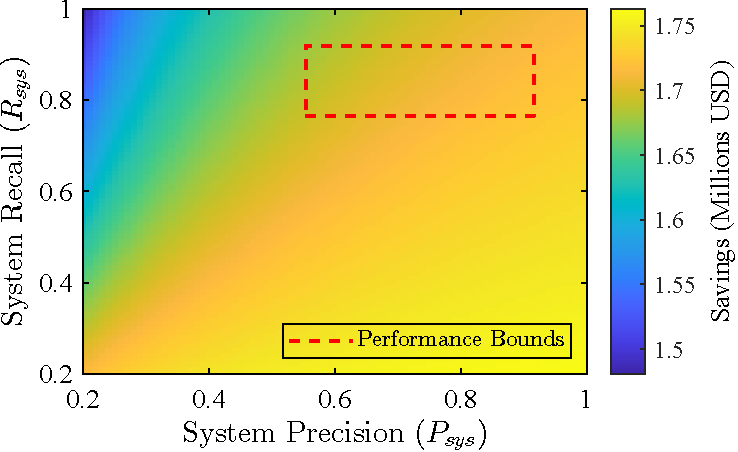
\includegraphics[width=0.5\textwidth]{figs/Rory/financial_savings.pdf} 
\caption[Operational Cost Savings as a Function of Computer Vision Performance]{Plot of Equation \ref{eq:drone_op_cost}. Operational cost savings of the proposed system over legacy systems for surveying and demining 1~km$^2$, varying with $P_{sys}$ and $R_{sys}$. The expected system performance from Section \ref{fusion_bounds} is the region inside the dashed rectangle.}
\label{fig:financial_savings}
\end{figure}


\subsection{Conclusion} \label{subsec:finance_conclusion}

This section suggests that the drone-based detection system proposed in this report offers significant financial benefits over legacy manual demining techniques. The operational costs are reduced by a factor of over 20$\times$, whilst the system is significantly faster. The improved precision means that the area flagged for clearance is much smaller than in legacy techniques, which causes a large reduction in the most significant part of the operational costs and times. These reductions in cost and time will enable more widespread demining operations, restoring large areas of productive land, and saving countless lives. 

Future work should investigate more accurate cost estimates. For the operational costs, more advanced YOLOv11 models (Section \ref{compvis_implementation}) should be trained on real world experimental data. The ANFIS network (Section \ref{fusion}) should be implemented, and the performance metrics $P_\text{sys}$ and $R_\text{sys}$ should be found by testing the entire system on a large dataset of unseen experimental data. This would give a more accurate picture of the system's financial viability, which would help in securing funding if the project were commercialised.


\include{Samuel/techstrat}

\newpage
\fancyhead[C]{Huirui Dai}
\setlength{\parindent}{0pt}

\section{Sustainability and Ethics} \label{sustainability & ethics}


\section{Conclusion} \label{conclusion}
\fancyhead[C]{Thomas Turner}
The work put forward is in line with our design and mission objectives. In this project we have shown the viability of the design at many levels. Sections \ref{section:Custom Hardware} and \ref{sec:bms} demonstrate how custom hardware will be used in order to meet the specific needs of the harsh operating conditions in line with the design goals and at lower cost than \gls{COTS} options. In Section \ref{sensor_hardware_data_acquisition} it is demonstrated how \gls{COTS} options can be used to gather high quality data needed for advanced data analysis specific to the task of removing anti-personal mines.

Section \ref{computervision} shows how the data acquired from the selected sensors can be used to detect anti-personal mines using simulations built with real world data from the region of interest using sensor fusion of \gls{GPR} and thermal data. Section \ref{sec:msp} demonstrates how missions will be planned to avoid obstacles and allow multi-agent drones to operate at peak efficiency using the innovative divide-and-cluster technique. 

Sections \ref{sec:euc} and \ref{Intra Communication} address how the device will communicate with the base station and between modules within the device considering modularity and redundancy at the forefront. The control system of the drone is also considered in Section \ref{sec:simcontrol} in order to optimise the stability and performance of the drone considering and considering multiple agents. 

In Section \ref{Return to Safety} a novel Return to Safety procedure is considered using adaptive control and path planning to attempt to land in safe regions if experiencing faults. Finally, project financing, sustainability, safety and risk, technology strategy are considered to ensure the long-term health of the project. 

In summary, from hardware to sensors to computer vision and mission planning all stages are considered to ensure the project is viable and effective.
\newpage
\fancyhead[C]{All Students}
\printbibliography{biblio}

% Appendix
% Essential content that interrupts the flow of the document can be placed here, e.g. technical drawings, detailed lists of equations used, etc.
\newpage
\addcontentsline{toc}{section}{Appendix}
\section*{Appendix}

\end{document}
